%\documentclass[aps,prb]{revtex4}
%\documentclass[aps,prb,twocolumn]{revtex4-1}
\documentclass[showpacs,aps,prb,reprint,superscriptaddress]{revtex4-1}
%\documentclass[showpacs,aps,prl,reprint,superscriptaddress,showkeys,floatfix,citeautoscript]{revtex4-1}
\usepackage{bm}
%\usepackage{subfig} % LUIS: This package messes with the captions.
\usepackage{graphicx}
\usepackage{graphics}
\usepackage{amsmath,amssymb,amstext}
\usepackage{amsfonts}

\usepackage{epstopdf}
\usepackage{hyperref}
\usepackage{hyperref}
\hypersetup{
    colorlinks,%
    citecolor=blue,%
    linkcolor=blue,%
    urlcolor=blue
}
%\usepackage{pgf}
\usepackage{tikz}\usetikzlibrary{petri}
%\usepackage{bbold}
%\usepackage{makeidx}
\newcommand{\TS}[1]{{$\rightarrow$ {\sl#1}}}
\newcommand{\LUIS}[1]{\textcolor{blue}{\fbox{Luis} {\sl#1}}}
\newcommand{\Jesus}[1]{\textcolor{red}{\fbox{Jesus} {\sl#1}}}
\begin{document}


\newcommand{\be}   {\begin{equation}}
\newcommand{\ee}   {\end{equation}}
\newcommand{\ba}   {\begin{eqnarray}}
\newcommand{\ea}   {\end{eqnarray}}
\newcommand{\ve}  {\varepsilon}

\newcommand{\nhat}{\hat{n}}
\newcommand{\veck}{\textbf{k}}
\newcommand\ep{\epsilon}
\newcommand\g{\gamma}
\newcommand\s{\sigma}
\newcommand\up{\uparrow}
\newcommand\dw{\downarrow}
\newcommand\down{\downarrow}
\newcommand{\ed}[1]{\ep_{d#1}}
\newcommand{\ket}[1]{\vert #1 \rangle}
\newcommand{\ann}{a^{\dagger}}
\newcommand{\dann}{d^{\dagger}}
\newcommand{\tdots}{t_{dots}}
\newcommand{\gammaA}[1]{\gamma_{A,#1}}
\newcommand{\gammaB}[1]{\gamma_{B,#1}}
\newcommand{\Green}[1]{G_{#1}(\omega) }

\newcommand{\GreenG}[2]{G_{#1}^{ #2} (\omega) }
%\newcommand{\bra}[3]{\langle {#3} \vert}

\newcommand{\super}{\vert \Delta \vert}





%%%%%%%%%%%%%%%%%%%%%%%%%%%%%%%%%%%%%%%%%%%%%%%%%%%%%%%%%%%%%%%%%%%%%%%%%%%%%%%
\title{ Manipulation of Majorana zero-modes using double quantum dots }

\author{Jesus D. Cifuentes}
\affiliation{Instituto de F\'{\i}sica, Universidade de S\~{a}o Paulo,
C.P.\ 66318, 05315--970 S\~{a}o Paulo, SP, Brazil}
\author{Luis G.~G.~V. Dias da Silva}
\affiliation{Instituto de F\'{\i}sica, Universidade de S\~{a}o Paulo,
C.P.\ 66318, 05315--970 S\~{a}o Paulo, SP, Brazil}

\date{ \today }

\begin{abstract}
\LUIS{We'll call them Majorana ``zero modes" instead of ``Majorana fermions", which relates more to elementary particles. }
\Jesus{Ok ;) }

Majorana zero modes (MZMs) appearing at the edges of topological superconducting wires are a promising platform for fault-tolerant quantum computation. Novel proposals use MZMs tunneling inside quantum dots (QDs) to implement quantum architectures because today’s precise experimental control over the QD parameters offers the unique possibility of manipulating the Majoranas inside multi-dot systems. The simplest case where Majorana manipulation is possible is in a double quantum dot (DQD). This model shows several possibilities for manipulation of MZM, including different geometric couplings such as linear forms of T-junctions. In this model we perform analytical (non-interacting) and numerical(interacting) quantum transport studies of the transition of the Majorana signature. By tuning the model parameters we show that it is possible to control the localization of the MZM inside the DQD. 




% Majorana fermions appearing at the edges of topological superconducting wires are a promising platform for fault-tolerant quantum computation. Novel proposals use Majorana modes tunneling inside quantum dots (QDs) to implement quantum architectures, because today’s precise experimental control over the QD parameters offers the unique possibility of manipulating the Majorana modes inside multi-dot systems. The simplest case where Majorana manipulation is possible is in a double quantum dot (DQD). So far, no complete analysis of this basic structure has been done. This  project fills this gap by realizing an exact quantum transport study of the effects of coupling a Majorana mode with a DQD. By tuning the model parameters we show that it is possible to control the localization of the Majorana signature in the DQD. 




\end{abstract} 
%\pacs{ APS does not use it anymore}
%\keywords{Quantum Spin-Hall effect, Edge transport, Topological insulators}

\maketitle


%%%%%%%%%%%%%%%%%%%%%%%%%%%%%%%%%%%%%%%%%%%%%%%%%%%%%%%%%%%%%%%%%%%%%%%%%%%%%%%v

%\pacs{ APS does not use it anymore}
%\keywords{Quantum Spin-Hall effect, Edge transport, Topological insulators}

\maketitle


%%%%%%%%%%%%%%%%%%%%%%%%%%%%%%%%%%%%%%%%%%%%%%%%%%%%%%%%%%%%%%%%%%%%%%%%%%%%%%%
\section{Introduction}
\label{sec:Intro}

\TS{Majorana zero modes in condensed matter systems: they have been found, several papers have been written about it and there has been much progress in distinguishing them from other sources of zero-bias peaks.}

The pursuit of Majorana quasi-particles in topological superconductors has attracted significant attention in the last decades.\cite{alicea_new_2012,beenakker_search_2013}  Since the first Kitaev's toy models \cite{kitaev_unpaired_2001,kitaev_fault-tolerant_2003} claiming promising applications to quantum computing, the field evolved rapidly towards physical realizations of the Kitaev chain.  The last few decades have been full of excitement as new technological innovations  allowed to document several times the observation of Majorana signatures. \citep{mourik_signatures_2012,das_zero-bias_2012,deng_anomalous_2012,nadj-perge_observation_2014,deng_majorana_2016,zhang_quantized_2018}  One of the most promising structures is the so-called Majorana wire, which recipe consists in growing semiconducting wires with strong-orbit-coupling over proximity-induced topological (p-wave) superconductors.  

These signatures are characterized by the emergence of robust zero modes localized at the edges of the material. However the observed Majorana zero-modes (MZM) have been found in superposition with other similar types of phenomenon such as the Kondo effect. \cite{lee_zero-bias_2012} The new experimental proposals foucus on distinguishing MZMs from other effects and performing braiding protocols,\cite{aasen_milestones_2016,sarma_majorana_2015,heck_coulomb-assisted_2012} a basic operation for topological quantum computing. 

\TS{MZMs in quantum dots can co-exist with Kondo peaks.}

One of the most promising methods to detect MZMs consists in attaching a quantum dot (QD) to the edges of a Majorana chain in the topological phase and executing transport measurements through the QD. \cite{liu_detecting_2011}  In such arrangement the MZM at the end of the chain leaks inside the ,QD \cite{vernek_subtle_2014} which produces a zero-bias conductance peak of half a quanta $\frac{e^{2}}{2h}$ through the dot. Recently, experiments including hybrid Majorana-QD systems have been performed. \cite{deng_majorana_2016} This method offers several advantages: 1) The qubit information  is not completely destroyed, in contrast to other detection methods such as tunneling spectroscopy. 2) If performed under the  Kondo temperature $T_k$ it allows the possibility of observing the  MZM co-existing with the Kondo peak, \cite{lee_kondo_2013,ruiz-tijerina_interaction_2015,gorski_interplay_2018} and methods for separating both effects 3) Today’s precise experimental control over the QD parameters offers the unique possibility of manipulating MZMs inside multi-dot systems. Hence bringing new lights into the design of quantum architectures. \cite{barkeshli_physical_2015,karzig_scalable_2017} 


\LUIS{Ok. Ref. \onlinecite{karzig_scalable_2017} is PRB of scalable designs: PRB \textbf{95} 235305 (2017). }




% In addition, under the Kondo regime 



%   In addition, the similarity of this phenomenon with the Kondo effect,\cite{hewson_kondo_1997,wilson_renormalization_1975} where the zero-bias conductance peak takes  $\frac{e^{2}}{h}$, motivated the study of combined Kondo-Majorana physics in this system. \cite{lee_kondo_2013,ruiz-tijerina_interaction_2015} This project revealed the existence of a region of parameters where bo
\TS{Here's what we did: quantum tunneling of a MZM into a double dot shows several possibilities for manipulation of MZM}


 The simplest case where Majorana manipulation is possible is in a double quantum dot (DQD). Tunneling Majorana modes in these basic structures have inspired theoretical studies \cite{silva_andreev_2016,ivanov_coherent_2017} and experimental setups confirming the observations of Andreev molecules \cite{su_andreev_2017}. Even though quantum tunneling of a MZM into a double dot shows several possibilities for manipulation of MZM,  there is still no complete analysis of the transitions of the Majorana signatures between the QDs in this model. 
 
 
 In this paper, we explore the different possibilities for Majorana manipulation in a device consisting of a DQD coupled to a MZM and a metallic lead (See Fig.\ \ref{fig:GenModel}). The simplicity of this model allows us to explore analytically different geometries of QD's from linear couplings to T-junctions (Fig.\ \ref{fig:MajoranaModels}). We considered both non-interacting and interacting regimes, observing major agreement between both approaches about the location of the Majorana signature.
 
 We performed a detailed study of the non-interacting DQD limit, by using Zubarev's procedure  \cite{zubarev_double-time_1960} to provide an algebraic procedure to calculate the spectral functions. For the interacting case, we resort to numerical renormalization group (NRG)\cite{bulla_numerical_2008} calculations for this model.
 While the non-interacting regime is suitable to obtain exact expressions for the Green function, the interacting case  shows how the Majorana signature co-exists with strongly correlated phenomena such as the Kondo effect \cite{hewson_kondo_1997} and RKKY interactions.   \cite{ruderman_indirect_1954,kasuya_theory_1956,yosida_magnetic_1957} 


This paper is organized as follows. In Sec.\ \ref{sec:modelmethods} we describe the model of a DQD coupled to a MZM and to a metallic lead, as well as the methods used.  The results are presented in section \ref{sec:results} where we compare the non-interacting density of states (DOS) \ref{subsect:non-int} with the low-energy  interacting results \ref{subsec:Interacting}. Finally, our conclusions are given in Sec.\ \ref{sec:Conclusions}.


  % So far, no complete analysis of this simple case has been done. The goal of this  project is to fill this gap by realizing a full quantum transport study of the effects of coupling a Majorana mode with a double quantum dot.  By tuning the QD gate voltages and the Majorana couplings we will be able to probe the mobility of the Majoranamodes through the dots. 




% \LUIS{In this paper, we ...} 
%   In this paper we  considered both interacting and non-interacting cases. For interacting systems we used a obtained the exact transport description . On non-interacting models we used a NRG approach.   We found that in symmetric couplings  In the non-interacting case, we confirmed that shifting the QD’s gate voltage induces the Majorana to tunnel only to the other dot. In addition, an indirect coupling of the second dot could cause destructive interference with the Majorana signature. In the interacting case,  the NRG simulations confirmed these results and showed that other interacting effects -  Kondo effect and RKKY interactions \cite{ruderman_indirect_1954,kasuya_theory_1956,yosida_magnetic_1957} - could coexist with the Majorana signatures. On the other hand, when only one QD is coupled to the leads and the other Dot is attached to the QD,  the Kondo effect is annihilated due to the destructive interference  generated by extra dot. \cite{dias_da_silva_transmission_2008} Our study includes how the Majorana mode interacts with these two effects.  
 


 % These experiments are performed at very low temperatures where the MZM could coexists with the  Kondo effect \cite{lee_kondo_2013,ruiz-tijerina_interaction_2015}.  


% Despite the positive experimental results, their is still certain skepticism about the existence . The zero mode could be the product of other phenomena  such as the Andreev bound states or even the Kondo effect. 

% Specially in the so called Majorana wires, where observations of zero modes have been documented   
%  To the date, extended experiments have documented the observation, of Majorana zero modes \cite{keylist}


%  Some proposals involve the coupling of quantum dot through superconductivity. 

% to create these materials consists in combining superconducting platform with a with strong-orbit coupling

%  % While some proposal include recreations of Kitaev model using quantum dot chains with superconducting couplings \cite

%  To the date, several experimental proposals have been put forward including InSb superconducting wire 
% {}


%  Majorana bound states appearing at the edges of topological superconductors to topological quantum computing
%  Kitaev's toy models  proposing the promising implementation of 

% the fields has evolved rapidly towards physical realizations of the Kitaev chain. To the date 

% The quasiparticle   is proposed to be one of the most promising approaches to fault tolerant quantum computing. Physical implementations of Kitaev's toy model such as Majorana wires and quantum dot chains 


% The quasi-particle initially proposed by Ettore Majorana 

% Predi

% The Majorana quasiparticle, which in Kitaev's toy model was predicted to appear at the edges of topological superconductors 
% ,
% as the real field solution of the Dirac equation describes a fermion which is its own antiparticle.

%  Though no fundamental particle with these characteristics have been found, 


% To the date no fundamental particle with this characteristic has been found. However, 
% Multiple advances in theoretical  followed by successful experimental have led to the observation of Majorana zero modes localized at the edges of topological superconductors. 
% During the last decade multiple advances in theoretical proposals and led to the detection of Majorana zero modes. 
% However,  theoretical research predicts that Majorana zero modes emerge at the boundary of certain type of topological superconductors. \citet{kitaev_unpaired_2001} 
% The induced topological protection and non-abelian statistics makes Majoranas it a promising candidate for  quantum computation
% To exploit this property a basic braiding  protocol 
% Topological algorithms depend on basic baiding  protocol 
% The Majorana quasiparticle as zero mode 
% The last few decades have been full of excitement as new technological innovations  allowed the observation of Majorana signatures in different topological materials. \citep{mourik_signatures_2012,das_zero-bias_2012,deng_anomalous_2012,zhang_quantized_2018} 


% Despite the positive experimental results, their is still certain skepticism about the existence . The zero mode could be the product of other phenomena  such as the Andreev bound states or even the Kondo effect. 

% Now thworetical proposals concentrate in that could differ the Majoranas from these phenomena and implementing the promising braiding protocol.




% This proposal got huge attention 


% \TS{What's next? Manipulation and braiding !}


% Despite the positive experimental results, their is still certain skepticism about the existence of  Majorana Fermions. One of the reasons  is that some properties of Majorana quasiparticles like the expected non-abelian statistics have not been measure. This property is of especial interest due to its promising applications in topological quantum computing. The braiding protocol based on  Majorana's non-abelian statistics is the key to  fault-tolerant quantum computation. \cite{kitaev_fault-tolerant_2003,sarma_majorana_2015} 

% Experimental proposals for braiding measurements have been  proposed  in one dimensional majorana chains.  The system inspired in the famous Kitaev toy model is a promising example of these topological superconductors.  The chain emulates a spinless p-wave superconducting wire. With the adequate combination of magnetic field,  superconducting gap and Rashba spin-orbit coupling  the wire enters into a topological phase in which zero-mode majorana bound states emerge. 

% This is a Majorana signature which produces half of the expected peak by a regular fermion. 



 
%  The idea of using hybrid quantum dot-Majoranaheteroestructures to implemtent quantum gates has aquired wide interest in the last years.  One of the insights of these structures is the posibility of manipunaling  Majoranas  in multidot systems by shifting the QD gate voltages and Hence the approach is suitable for the implementation of braiding procedures . The simplest system where Majorana manipulation is possible is  a  double quantum dot (DQD) coupled to a Majoranachain. So far, no complete analysis of this simple case has been done. The goal of this  project is to fill this gap by realizing a full quantum transport study of the effects of coupling a Majorana mode with a double quantum dot.
 



% In the last few decades the interest in the so called Majorana fermions has been increasing. The particle proposed by the physicist Ettore Majorana  as the real field solution of the Dirac equation describes a fermion which is its own antiparticle, hence it has no charge nor mass. To the date no fundamental particle with these characteristics has been found. However,  theoretical research predicts that Majorana Fermions emerge as quasi-particles at the boundary of certain topological superconductors. \citet{kitaev_unpaired_2001} Recently, the new technological innovations  allowed the observation of Majorana signatures in different topological materials. \citep{mourik_signatures_2012,das_zero-bias_2012,deng_anomalous_2012,zhang_quantized_2018}

% Despite the positive experimental results, their is still certain skepticism about the existence of  Majorana Fermions. One of the reasons  is that some properties of Majorana quasiparticles like the expected non-abelian statistics have not been measure. This property is of especial interest due to its promising applications in topological quantum computing. The braiding protocol based on  Majorana's non-abelian statistics is the key to  fault-tolerant quantum computation. \cite{kitaev_fault-tolerant_2003,sarma_majorana_2015} 

% % Experimental proposals for braiding measurements have been  proposed  in one dimensional majorana chains.  The system inspired in the famous Kitaev toy model is a promising example of these topological superconductors.  The chain emulates a spinless p-wave superconducting wire. With the adequate combination of magnetic field,  superconducting gap and Rashba spin-orbit coupling  the wire enters into a topological phase in which zero-mode majorana bound states emerge. 

% A promising method to detect Majorana modes consists in attaching a quantum dot (QD) to the edges of a Majorana chain in the topological phase and executing transport measurements through the QD. \cite{liu_detecting_2011}  The Majorana mode at the end of the chain then leaks inside the QD \cite{vernek_subtle_2014} which produces a zero-bias conductance peak of half a quanta $\frac{e^{2}}{2h}$ through the dot. This is a Majorana signature which produces half of the expected peak by a regular fermion.  Recently, experiments including hybrid Majorana-QD systems have been performed. \cite{deng_majorana_2016}  In addition, the similarity of this phenomenon with the Kondo effect,\cite{hewson_kondo_1997,wilson_renormalization_1975} where the zero-bias conductance peak takes  $\frac{e^{2}}{h}$, motivated the study of combined Kondo-Majorana physics in this system. \cite{lee_kondo_2013,ruiz-tijerina_interaction_2015} This project revealed the existance of a region of parameters where both, Kondo and Majorana physics, coexist. 

% This idea has turned on new lights into the design of quantum architectures, \cite{barkeshli_physical_2015,karzig_scalable_2017}  because today’s precise experimental control over the parameters of QDs - energy levels, tunneling couplings, etc. - offers the unique possibility of manipulating the Majorana modes inside multi-dot systems. The simplest case where Majorana manipulation is possible is in a double quantum dot. So far, no complete analysis of this simple case has been done. The goal of this  project is to fill this gap by realizing a full quantum transport study of the effects of coupling a Majorana mode with a double quantum dot.  By tuning the QD gate voltages and the Majorana couplings we will be able to probe the mobility of the Majoranamodes through the dots. 
 
% %  The idea of using hybrid quantum dot-Majoranaheteroestructures to implemtent quantum gates has aquired wide interest in the last years.  One of the insights of these structures is the posibility of manipunaling  Majoranas  in multidot systems by shifting the QD gate voltages and Hence the approach is suitable for the implementation of braiding procedures . The simplest system where Majorana manipulation is possible is  a  double quantum dot (DQD) coupled to a Majoranachain. So far, no complete analysis of this simple case has been done. The goal of this  project is to fill this gap by realizing a full quantum transport study of the effects of coupling a Majorana mode with a double quantum dot.
 
 
%   We  considered both interacting and non-interacting cases. For interacting systems we used a obtained the exact transport description . On non-interacting models we used a NRG approach.   We found that in symmetric couplings  In the non-interacting case, we confirmed that shifting the QD’s gate voltage induces the Majorana to tunnel only to the other dot. In addition, an indirect coupling of the second dot could cause destructive interference with the Majorana signature. In the interacting case,  the NRG simulations confirmed these results and showed that other interacting effects -  Kondo effect and RKKY interactions \cite{ruderman_indirect_1954,kasuya_theory_1956,yosida_magnetic_1957} - could coexist with the Majorana signatures. On the other hand, when only one QD is coupled to the leads and the other Dot is attached to the QD,  the Kondo effect is annihilated due to the destructive interference  generated by extra dot. \cite{dias_da_silva_transmission_2008} Our study includes how the Majorana mode interacts with these two effects.  
 
 
%  When both dots are coupled to the leads the Double Quantum Dot exhibits an antiferromagnetic interaction known as  Ruderman-Kittel-Kasuya-Yosida (RKKY) interaction. On the other hand, when only one QD is coupled to the leads and the other Dot is attached to the QD,  the Kondo effect is annihilated due to the destructive interference  generated by extra dot \cite{dias_da_silva_transmission_2008}. Our study includes how the Majorana mode interacts with these two effects.  



%  One of the insights of this method is that the information of the qubit is not completely destroyed as in other methods like tunneling spectroscopy. 
%  When Majoranas are connected to multidot systems it is possible to manipulate the Majorana mode inside the QDs  by tuning the gate voltage and  tunnel couplings. This fa

%following the prescription by \citet{oreg_helical_2010} and \citet{lutchyn_majorana_2010}.   

% Despite the positive experimental results, the proof One of the most promising aplications of Majorana Fermions is the implementaition of  braiding procedures  which are the key to implement fault-tolerant quantum computers. 
% Most of the experiments have been based on tunneling spectroscopy in junctions between TS and non metallic (NM) leads, where resonances have been observed at zero energy, consistent with the presence of Majorana zero\textendash energy modes. A downside of the tunneling spectroscopy technique  is that it probes not only the end of the Topological Superconductor(TS), but its bulk as well ,
% which completely destroys the qubit information. A less destroying



% In addition, the use of QDs favors the manipulation of the Majorana mode through the shifting of the dot gate voltage and the hopping parameters.

 
 




% Then the Majorana  as proposed by  \citet{liu_detecting_2011} and consists in coupling a quantum dot (QD) to the end of a TS. The analysis performed by Liu of this model revealed a  when the TS is in the topological phase,  which a signature of
% Majorana physics. On 2014, \citet{vernek_subtle_2014} showed that the Majorana Bound State at the end of the TS actually leaks inside the QD , which produces the conductance decay. and the model has been based for braiding experimental proposal
% To the date experimental procedures have been put forward. ery recently the first evidence of Majorana end states
% in TS has been found in multiple experiments


% as quasi-particles in certain types of topological materials have increased. The Majoranas are fermions that are their own anti-particle, hence have no charge nor mass. 
% The Majorana is predicted to be one of the most suitable alternatives to implement fault-tolerant quantum computers. Many experiments showing Majorana signatures in the conductivity have been performed. 
% Basics of Majorana Bound states:  zero-energy edge states in 1D topological superconductors.  

% Discovery on semiconductor nanowires \cite{Oreg:Phys.Rev.Lett.:177002:2010,Lutchyn:Phys.Rev.Lett.:77001:2010,Alicea:Reports:2012} etc. Experimental results \cite{Mourik:Science:1003:2012} \LUIS{Add others.}


% Leaking of Majorana to a QD: \cite{vernek_subtle_2014}, Interplay of Kondo and Majorana\cite{ruiz-tijerina_interaction_2015} Important results: Majorana and Kondo co-exist in the quantum dot even if the dot is non-topological.

% More recent experimental results: Deng et al. \cite{deng_majorana_2016} attached a QD to the end of a nanowire.

% Here we study the coupling of a MBS to a \emph{double} quantum dot system. 

% \TS{Punchline} Multidot systems offer the possiblity of ``moving'' Majoranas aroung using gate voltages and couplings. ossibility of Majorana braiding. Here, we study the simplest case, which is a double dot system.

%%%%%%%%%%%%%%%%%%%%%%%%%%%%%%%%%%%%%%%%%%%%%%%%%%%%%%%%%%%%%%%%%%%%%%%%%%%%%%%
\section{Model and methods}
\label{sec:modelmethods}


We consider the setup shown in Figure \ref{fig:GenModel}, in which a single MZM $\gamma_1$ located at the edge of a 1D topological superconductor is coupled to a double quantum dot (DQD) attached to a single metallic lead. The Hamiltonian of the entire system can be expressed as:
%
\begin{equation}
H=H_{\rm DQD}+H_{\rm lead}+H_{\rm DQD-lead}+H_{\rm M-DQD} 
\label{eq:Model}
\end{equation}
%
where the different terms describe, respectively, the (interacting) DQD, the (non-interacting) metallic lead, and the DQD-lead and DQD-MZM couplings:
%The interacting Anderson Model describes the DQD-lead system  
%d_{i\sigma}^{\dagger}d_{i\sigma}
\begin{align}
%\begin{split}
    H_{\rm DQD} =& \!  \sum_{\substack{i\!=\! 1,2 \\ \sigma \!=\! \dw , \up }} \left(\epsilon_{di}+\frac{U_i}{2}\right)\hat{n}_{i\sigma} + \frac{U_i}{2}\left(\sum_{\sigma} \hat{n}_{i\sigma}-1\right)^{2} \\ \nonumber
& + \sum_{\sigma} \tdots(\dann_{1\sigma}  d_{2\sigma}+\dann_{2\sigma}  d_{1\sigma}) \; , \\ \nonumber
H_{\rm lead} =&  \sum_{\mathbf{k}\sigma }\epsilon_{\mathbf{k}}c_{\mathbf{k}\sigma}^{\dagger}c_{\mathbf{k}\sigma }  \; , \\ \nonumber
H_{\rm DQD-lead} =&  \sum_{\mathbf{k}\sigma }\sum_{i\!=\!1,2 }V_{i\textbf{k}} c_{\mathbf{k}\sigma }^{\dagger}d_{i\sigma}+V^*_{i\textbf{k}} d_{i\sigma}^{\dagger}c_{\mathbf{k}\sigma } \; , \\ \nonumber
H_{\rm M-DQD} =&  \sum_{i=1}^2t_{i} \left(d_{i\downarrow}^{\dagger}\gamma_{1}+\gamma_{1}d_{i\downarrow}\right) \; .
%
\label{eq:H_DQD}
\end{align}


%

In the equations above, $\ed{i}$ is the energy level of dot $i$, $U_i$ is the Coulomb repulsion and $\tdots$ is the coupling parameter between both QDs. The operator $\dann_{i\sigma}$ creates a particle in dot $i$ with spin $\sigma$ and $\hat{n}_{i\sigma}:=d_{i\sigma}^{\dagger}d_{i\sigma}$ is the particle number operator of state $i$.  $c_{\mathbf{k}\sigma }^{\dagger}$ is the creation operator a particle with momentum $\mathbf{k}$ and spin
$\sigma$ in the lead.  $\epsilon_{\mathbf{k}l}$ is the corresponding energy
 and $V_i(\textbf{k})$ describes the tunneling coupling between the lead and dot $i$ . \\


%-----------F I G U R E  1 ------
\begin{figure}[t]
\begin{center}
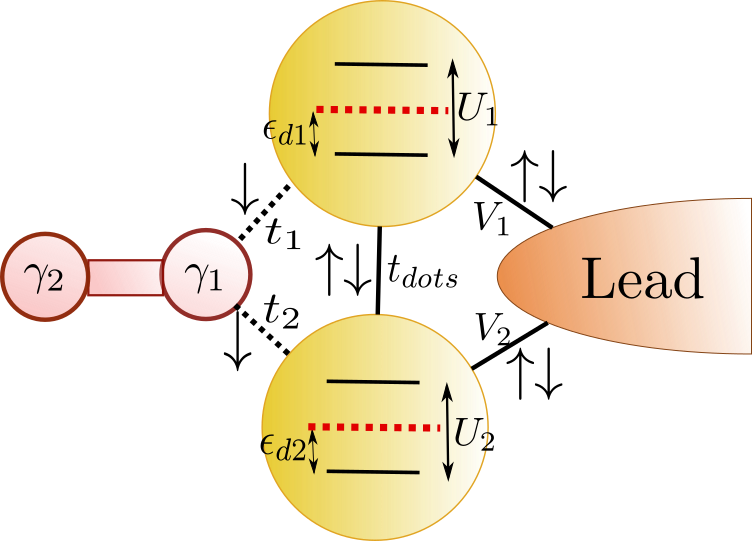
\includegraphics[scale=0.4]{Graficos/GenModel.png}
\end{center}
\caption{ Model for the DQD-Majorana system. Solid lines: Hopping interactions ($t_{dots}$: inter-dot coupling , $V_1,V_2$ couplings of QD1 and QD2 with the lead. ). Dashed lines: Majorana spin-$\dw$ effective couplings \eqref{eq:H_MDQD} $t_1,t_2$. The atomic energy levels appear inside each QD $\ep_1, \ep_2$ are tuned by the gate voltages. The coulomb interaction is represented by $U_1,U_2$.  The red dashed horizontal lines represent the Fermi level.
}
%
\label{fig:GenModel}
\end{figure}
%-----------E N D  F I G U R E  1 ------


% To model the interaction between the DQD and the Majorana Mode we define the Majorana operators as the

It is sometimes useful to recast the last term in Eq.\ (\ref{eq:Model}) in terms of (Dirac) fermionic operators. Following Refs. \onlinecite{lee_kondo_2013,ruiz-tijerina_interaction_2015}, we choose to write the Majorana zero modes $\gamma_1$ and $\gamma_2$ as a superposition of the creation ($f^{\dagger}_\dw$) and annihilation ($f^{ }_\dw$) operators of a spin $\dw$ fermion:
%
\begin{equation}
    \gamma_1 := \frac{1}{\sqrt{2}} \left( f^\dagger_{\dw} + f_{\dw}\ \right) \; , \gamma_2 := \frac{i}{\sqrt{2}} \left( f^\dagger_{\dw} - f_{\dw} \right) \; . \label{eq:MajOp}
\end{equation}


In this representation, the effective coupling between the MZM $\gamma_1$ and the DQD becomes:
%by attaching $\gamma_1$ with the spin-$\dw$ channel in the DQD:

%H_{TS} & = & 2\epsilon_{m}\gamma_{1}\gamma_{2}\nonumber \\
\begin{eqnarray}
	H_{\rm M-DQD} & = &  
	%\sum_{i=1}^2t_{i} %\left(d_{i\downarrow}^{\dagger}\gamma_{1}+\gamma_{1}d_{i\downarrow}\right) + %\epsilon_M \gamma_1\gamma_2. 
	% \\
\sum_{i}t_{i} \left(d_{i\downarrow}^{\dagger}f^\dagger_{\dw} + 
	 f_{\downarrow}d_{i\dw} +d_{i\downarrow}^{\dagger}f_{\dw}+
	 f_{\downarrow}^{\dagger} d_{i\downarrow}\right) \; , 
	\label{eq:H_MDQD}
\end{eqnarray}
where $t_i$ is the coupling parameter between the Majorana mode and QD $i$. %$\epsilon_m$ is the coupling energy between both Majorana modes.

Given the model, the quantities of interest to be calculated are the spein-resolved spectral functions (or, equivalently, the local density of states) of the quantum dots. These will give us information of the presence/absence of MZMs ``leaking'' from the edge of the TS into the dots \cite{liu_detecting_2011,vernek_subtle_2014,ruiz-tijerina_interaction_2015}. As usual, the spectral function for spin $\sigma$ in dot $i$ is defined as:
%
%
\begin{equation}
    \rho_{i \sigma}(\omega)\equiv-\frac{1}{\pi} \textrm{Im} \left[G_{d_{i \sigma},d_{i \sigma}^\dagger}(\omega)\right].
    \label{eq:SpecFunc}
\end{equation}
%
where $G_{d_{i \sigma},d_{i \sigma}^\dagger}(\omega) \equiv \langle\langle d_{i \sigma},d_{i \sigma}^\dagger} \rangle \rangle_\omega$ is the retarded (diagonal) Green's function involving dot $i$ operators $d_{i \sigma}$ and $d_{i \sigma}^\dagger}$. Next, we describe the procedures for calculating  $\rho_{i \sigma}(\omega)$ in the regimes of weak ($U_i \ll V$) and strong ($U_i \! \gg\! V$) electron-electron interaction in the dots.


% ----------------------------------------------------------------------------------------------------------
 % ----------------------------------METHODS------------------------------------------------------------------
% --------------------------------------------------------------------------------------------------------------
% \newpage

\subsection{Non-interacting limit: Equations of motion }
\label{sec:non-interactingMethods}

In the non-interacting limit ($U_i\!=\!0$), we can obtain analytic expressions for the spectral densities defined in Eq.\ (\ref{eq:SpecFunc}). Using Zubarev's equation of motion (EOM) approach \cite{zubarev_double-time_1960}, we can derive  exact expressions for the Green functions associated to both quantum dot operators $(\Green{d_1d^\dagger_1},\Green{d_2d^\dagger_2})$. 

The detailed procedure is described in Appendix \ref{sec:Appendix_alg}. The EOM  equations define a $9 \times 9$ linear system where the Hamiltonian parameters $(t_1,t_2,\epsilon_1 \ldots)$ and the energy $\omega$ are taken as algebraic variables. The solution for these types of equations is a polynomial fraction of the same degree, which makes it difficult to provide an exact solution using either analytic or numerical methods. 

To bypass this problem, we associated the quantum dot system to a ``flow graph'' and used a Graph-Gauss-Jordan elimination process \cite{spielman_algorithms_2010}.  This method proved to be efficient in solving complex transport systems of coupled Green's functions since the graph structure allows us to identify minimum cutting points  and create an algorithmic representation of the Green function. 

\LUIS{Stopped here. To be continued...}

% This idea also brings new perspectives to the theory of Majorana systems since the Majorana fermion is an articulation point in the graph that communicates creation and annihilation operators

At the end, we obtained the following analytical expression
\begin{equation}
    G_{{d_{1\downarrow},d_{1\downarrow}^{\dagger}}}\left(\omega\right)=\frac{1}{\omega-\epsilon_{DQD}^{+}-\frac{\left\Vert T_{+}\right\Vert ^{2}}{\omega-\epsilon_{M2}-\frac{\left\Vert T_{-}\right\Vert ^{2}}{\epsilon_{DQD}^{-}}}}.
    \label{eq:Green_NonInteracting}
\end{equation}
\noindent Where
\begin{equation}
    \epsilon_{DQD}^{\pm}=\pm\epsilon_{1}+\sum_{\mathbf{k}}\frac{V_{1}V_{1}^{*}}{\omega-\epsilon_{\mathbf{k}}}+\frac{\left\Vert \pm t_{dots}+\sum_{\mathbf{k}}\frac{V_{1}V_{2}^{*}}{\omega-\epsilon_{\mathbf{k}}}\right\Vert ^{2}}{\omega\pm\epsilon_{2}-\sum_{\mathbf{k}}\frac{V_{2}V_{2}^{*}}{\omega-\epsilon_{\mathbf{k}}}}, \label{eq:epDQD}
\end{equation}
\noindent 

\begin{equation}
    T_{\pm}=\pm t_{1}\pm t_{2}\frac{\left(\pm t_{dots}+\sum_{\mathbf{k}}\frac{V_{1}V_{2}^{*}}{\omega-\epsilon_{\mathbf{k}}}\right)}{\omega\pm\epsilon_{2}\pm\sum_{\mathbf{k}}\frac{V_{2}V_{2}^{*}}{\omega-\epsilon_{\mathbf{k}}}}, \label{eq:T+-}
\end{equation}

\noindent and
\begin{equation}
    \epsilon_{M2}=\omega-\epsilon_{M}-\frac{\frac{\omega}{\omega+\epsilon_{M}}\left\Vert t_{2}\right\Vert ^{2} } {\omega-\epsilon_{2}-\sum_{\mathbf{k}}\frac{V_{2}V_{2}^{*}}{\omega-\epsilon_{\mathbf{k}}}}-\frac{\frac{\omega}{\omega+\epsilon_{M}}\left\Vert t_{2}\right\Vert ^{2}}{\omega+\epsilon_{2}-\sum_{\mathbf{k}}\frac{V_{2}V_{2}^{*}}{\omega+\epsilon_{\mathbf{k}}}}. \label{eq:M2}
\end{equation}



% Note also that the spin-$\up$ green functions  can be obtained by replacing the Majorana couplings $t_1,t_2 = 0$.

\noindent On the other hand the spin-$\up$ DOS, which is not coupled to the MZM, can be obtained by taking $t_1,t_2 = 0$, hence giving
\begin{equation}
    G_{{d_{1\uparrow},d_{1\uparrow}^{\dagger}}}\left(\omega\right)=\frac{1}{\omega-\epsilon_{DQD}^{+}}.
    \label{eq:Green_NonInteracting}
\end{equation}


The final results will depend on the broadening parameter of QD $i$ with the lead $(\Gamma_i)$. This broadening satisfies the equation

\begin{equation}
   -i\Gamma_i = \lim_{s\rightarrow 0} \sum_{\boldsymbol{k}}\frac{V_{i}^{*}V_{i}}{\omega+ is -\epsilon_{\boldsymbol{k}}}.
\end{equation}
\noindent By convention we take $\Gamma_1$ as the energy unit for the rest of the project. Finally we compute the DOS 
\begin{equation}
    \rho_{1\sigma}(\omega)=-\frac{1}{\pi} \textrm{Im} \left[G_{d_{1\sigma},d_{1\sigma}^\dagger}(\omega))\right].
    \label{eq:Density of States}
\end{equation}
\noindent Similar results can be obtain for the DOS of the second $\rho_{2\sigma}$ by exchanging the indexes $1$ and $2$ in equation \eqref{eq:Green_NonInteracting}. 

The density of states provides significant information about the presence of a Majorana zero modes in the dot. We characterize the Majorana signature by a robust zero-mode with two possible heights:
 \begin{itemize}
         \item \textbf{Type I: }  The spin-$\dw$ DOS is the half of the spin-$\up$ DOS  at the Fermi energy $(\rho_\dw(0)=\rho_\up(0))$. 
         \item \textbf{Type II: } A spin-$\dw$ zero mode of height $ \rho_\dw(0) = \frac{0.5}{\pi  \Gamma_1}$. 
     \end{itemize}
In our results we observe several times these two types of signatures. Type I often appears when there is a zero-mode in the spin-$\up$ DOS. Type II emerges in the other situations. 
 % Considering that only the spin-$\downarrow$ channel is connected to the Majorana mode and that the spin-$\uparrow$and spin-$\downarrow$ channels are decoupled in non-interacting systems, the existence of this second type of Majorana signature is intriguing.   



\subsection{Interacting limit: Wilson's NRG }
\label{sec:NRG-interacting}

% For the interacting case, we used the Numerical Renormalization Group (NRG) approach \cite{wilson_renormalization_1975,sindel_numerical_2005,bulla_numerical_2008}.

The Numerical Renormalization Group (NRG) \cite{wilson_renormalization_1975,sindel_numerical_2005,bulla_numerical_2008} is the most successful methods to study interacting quantum impurity models. In this project, the impurity is described by the DQD attached to a Majorana mode. Our code a coulomb repulsion factor of $U =17.3\Gamma_1$ in both dots and a cut-off energy of $D=2U=34.6\Gamma_1$. The spacing with other energy levels is assumed to be higher than $D$, such that only the two coulomb states are relevant for the system dynamics. Particle-Hole-Symmetry at each dot is obtained when  $\epsilon_i = \frac{U}{2}$ in both dots. At this point, each dot has an odd number of electrons, hence, at sufficiently low temperature the system will exhibit the characteristic Kondo peaks at the Fermi energy \citet{wilson_renormalization_1975}. The coexistence of Kondo and Majorana zero modes is still a point of contention in the area and one of the objectives of this part of the project


% Observing how the Kondo-effect interacts with the Majorana signature in the double quantum dot is also an insight of this project. 


To  improve the efficiency of the code we used the symmetries of the system to maintain a block structure during NRG's iterative diagonalization process. This model preserves the spin-$\up$ particle number $\hat{N}_\up$ and the spin-$\dw$ parity $\hat{P}_\dw = \pm $ ($+$ even, $-$ odd). The spin-$\dw$ particle number is not preserved due to superconducting-type Majorana coupling  \eqref{eq:H_MDQD} . The initial Hamiltonian is organized in blocks according to these symmetries. This block structure is preserved during the entire iteration process \cite{bulla_numerical_2008}. To compute the spectral functions, we use the density matrix renormalization group (DM-NRG)  \cite{hofstetter_generalized_2000} in combination with the renown Z-trick method \cite{oliveira_generalized_1994}, which improves spectral resolution at high energies.
  
%   To unify the units of the interacting and non-interacting case we pick $U=8.69\Gamma_1$ and we let $D = 2U_1=17.3 \Gamma_1$.
 \section{Results \label{sec:results}}
  %-----------F I G U R E  MODELS ------
\begin{figure}[h]
	\begin{center}
	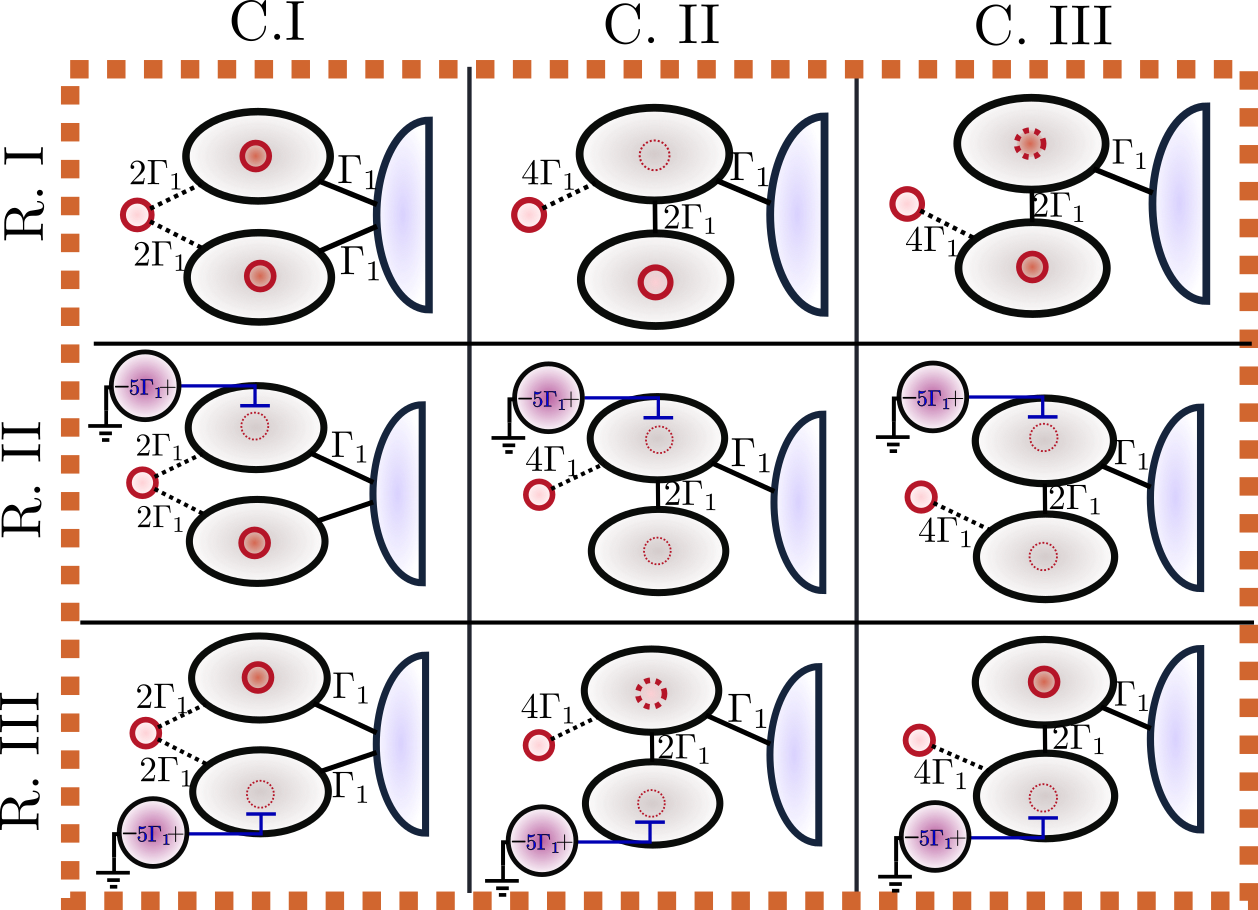
\includegraphics[scale=0.5]{Graficos/MajoranaModels.png}
	\caption{\label{fig:MajoranaModels}  Cases of study: (a) Symmetric coupling of the DQD to the lead and the MZM. No inter-dot coupling. (b)\&(c) Indirect coupling of the second QD through the first dot. The Majorana is coupled to the (b) first dot or to the (c) second dot. 
	}
	%
\end{center}
\end{figure}
%-----------E N D  F I G U R E  3 ------

%-----------F I G U R E  3 ------
	\begin{figure}[bt]
		\begin{center}
		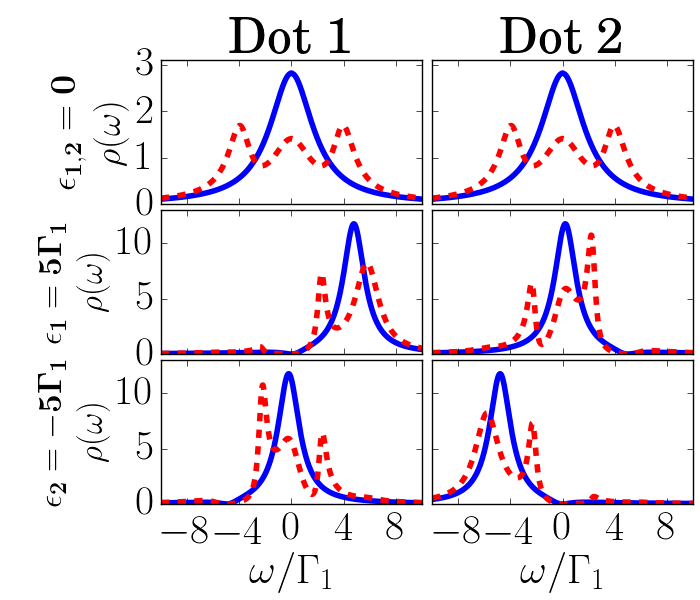
\includegraphics[scale=0.48]{Graficos/t1=t2.png}
		\caption{ \label{fig:t1=t2}  Non-interacting DOS in the symmetric coupling setup (Fig.\ref{fig:MajoranaModels}(a)) at each QD. First column: Dot 1. Second column: Dot 2. The gate voltages vary at each row.  First row: Zero gate voltages $\ep_1=\ep_2=0$. Second row: $\ep_1=5\Gamma_1, \ \ep_2 =0$.  Third row: $\ep_1=0, \ \ep_2 =-5\Gamma_1$.  Bold blue lines: Spin-$\up$ DOS. Thin red lines: Spin-$\dw$ DOS. The insets at the right show which dot carries a Majorana signature, represented by a red dashed circle. Upper: First dot. Lower: Second dot. 
		}
		%
	\end{center}
	\end{figure}
%-----------E N D  F I G U R E  3 ------

We call MZM manipulation to the "movements" attributed to the Majorana signature under the tunning of the dot gate voltages $( \epsilon_1 , \epsilon_2 )$. This manipulation process is performed in three different set ups that are presented in Fig.\ref{fig:MajoranaModels} with definite values of $\Gamma_2$, $t_dots$, $t_1$ and $t_2$. In configuration (a), we coupled the QD symmetrically to the lead and the Majorana mode. With this setup we expect to break the localization of the MZM which should split and tunnel into both dots. In setups (b) and (c) we coupled the second dot indirectly through the first dot. Hence, quantum  interference should split the zero mode in two states. Our objective is to observe what occurs with the Majorana signature in this situation. There are two options to connect the MZM in this situation. Attached it directly through the first dot (b) or indirectly through the second dot (c). 

     \subsection{MZM manipulation in non-interacting quantum dots \label{subsect:non-int}}

     % In non-interacting dots $(U=0)$, the density of states at each dot can be obtained from equation \eqref{eq:Density of States} by replacing the green function at \eqref{eq:Green_NonInteracting}. 
     

      %-----------F I G U R E  4 ------
\begin{figure}[bt]
\begin{center}
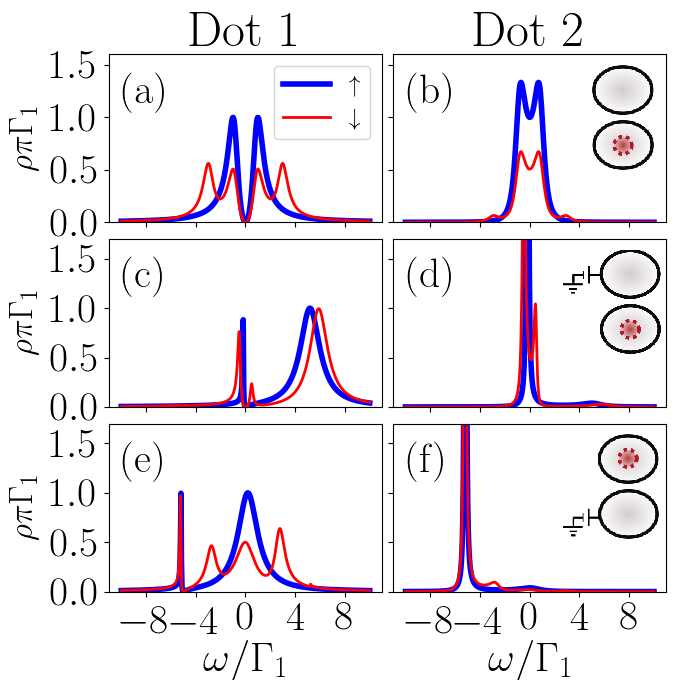
\includegraphics[scale=0.48]{Graficos/t1>0.png}
\caption{  \label{fig:t1>0} The same as in FIG.\ref{fig:t1=t2} for the non-interacting DOS of the setup in Fig.\ref{fig:MajoranaModels}(b) 
}
%
\end{center}
\end{figure}
%-----------E N D  F I G U R E  4 ------


 	 The non-interacting results for setups (a),(b) and (c) of FIG.\ref{fig:MajoranaModels} are shown at figures FIG.\ref{fig:t1=t2}, FIG.\ref{fig:t1>0} and FIG.\ref{fig:t2>0} respectively. Each figure depicts the DOS of dot $1$(left) and dot $2$(right). The gate voltage is initially $0$ in both dots at the first row. In the second row the gate voltage is turned on to  $\epsilon_1 = 5\Gamma_1$ in the first dot and remains at $\epsilon_2 = 0$ in the second dot. In the third row the first dot's voltage is off $\epsilon_1=0$ and we switch on the second dot with a negative voltage of $\epsilon_2 = -5\Gamma_1$. The insets at each row shows which dots exhibit Majorana signatures, depicted by a red dashed circle inside the dot. These images will continuously change under the tuning of gate voltages which represents the manipulation of the Majorana signature.


 %-----------F I G U R E  5 ------
\begin{figure}[bt]
\begin{center}
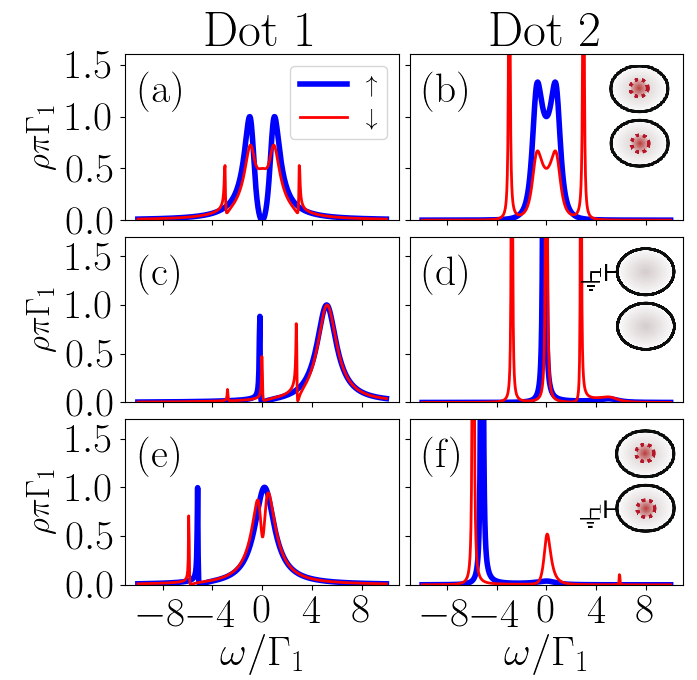
\includegraphics[scale=0.48]{Graficos/t2>0.png}
\caption{  \label{fig:t2>0} The same as in FIG.\ref{fig:t1=t2} for the non-interacting DOS of the set up in Fig.\ref{fig:MajoranaModels}(c) .
}
%
\end{center}
\end{figure}
%-----------E N D  F I G U R E  5 ------
     
    
     In FIG.\ref{fig:t1=t2} we observe the results for the symmetric coupling setup FIG.\ref{fig:MajoranaModels}(a). In the particle hole symmetric case (first row) the DOS is equal in both dots. Note that that the spin-$\dw$ (Thin red line) DOS is the half of the spin-$\up$ (Bold blue line) DOS at the Fermi energy $(\rho_\dw(0) = \frac{1}{2}\rho_\up(0))$. This type II Majorana signature is similar to the one observed when a single dot is coupled to a Majorana mode. \cite{liu_detecting_2011} We may conclude that the Majorana in tunneling inside both dots breaking the localization of the MZM. If a positive or negative gate voltage is induced in one of the dots, as shown in the second and third row of Figure \ref{fig:t1=t2}(c)-(f),  the Majorana zero mode vanishes from that dot. Meanwhile the density of states in the other dot increases while preserving the Majorana signature. This means that the MZM is actually being induced to "leave" this dots and leak into the other dot by the gate voltage activation. This first example of MZM manipulation. 

    Another example of MZM manipulation occurs when the second dot is not directly connected to the lead. In this case, the inter-dot tunneling generates quantum interference which finally destroys the central peak as observe in FIG.\ref{fig:t1>0}(a) at the spin-$\up$ DOS . The spin-$\dw$ channel at FIG.\ref{fig:t1>0}(a), which is coupled to the MZM, does not exhibit the characteristic Fermi peak either. Instead, the one half Majorana signature at the Fermi energy $(\rho_\dw(0) = \frac{1}{2}\rho_\up(0))$ appears clearly inside the second dot FIG.\ref{fig:t1>0}(b). This situation prevails when the first dot's gate voltage is turned on FIG.\ref{fig:t1>0}(c)\&(d). While the first dot does not seem to exhibit any type of Majorana signature, the second dot's spin-$\dw$ DOS exhibits a robust zero-mode of height $\frac{0.5}{\pi \Gamma}$. The results are more exciting when the second dot's gate voltage is turned on in FIG.\ref{fig:t1>0}(e)\&(f). These figures clearly show how the MZM, previously localized at the second dot, is induced to leave this dot and returned onto the first dot. Moreover, the DOS of spin-$\up$ and spin-$\dw$ channels are very similar to the spectral densities observed at FIG.\ref{fig:t1=t2}(d)(e), which means that the previous interference pattern has disappeared due to the presence of this gate voltage. 

    The results of the third configuration FIG.\ref{fig:MajoranaModels}(c) appear in FIG.\ref{fig:t2>0}. Contrary to what was observed in the previous case, this time the Majorana signature is not destroyed by the interference but instead, the  $\frac{0.5}{\pi \Gamma}$-height MZM emerges indirectly in the first dot. This is a perfect way to separate the Majorana's spin-$\dw$ DOS from the central spin-$\up$ zero-mode which is still destroyed by the interference. In addition, the second dot still exhibits a type I Majorana signature as observed in FIG.\ref{fig:t2>0}(b). In the second row we observe that turning on the gate voltage in dot $1$  destroys the Majorana signature in both dots FIG.\ref{fig:t2>0}(c)(d). On the other hand, if the second dot's voltage is switched both dots will preserve their Majorana signature (QD1:type I, QD2: type II), while the spin-$\up$ quantum interference vanishes in the first dot. 

    % With the MZM coupled only to the second dot, it is impressive that a Majorana signature of height $\frac{0.5}{\pi \Gamma}$ appears it the first dot despite there is no direct connection  between them. 
    % On the other hand, if the Majorana mode is attached to the second dot in the previous arrangement, then both dots will exhibit a majorana signature. However, the signature in dot 1 is different from the others. The spin-$\dw$ DOS reveals the emergence of a zero mode with height close to $5.2$ (such that $\pi  \Gamma_1 \rho_\dw(0) = 0.5$). However the spin-$\up$ DOS remains equal to $0$. This new type of majorana signature is the result of an indirect connection between QD1 and the majorana mode attached t the second dot. As in the previous case, turning on the gate voltage in dot $1$ destroys the majorana signature in both dots. Instead, if the gate voltage in dot $2$ is turned on, both dots will preserve the Majorana signature. 

    %  \noindent The state of these signatures for each of these stated is depicted in FIG.\ref{fig:MajoranaModels}. A solid filled red circle inside the dot represents the appearance of a Type I Majorana signature, on the othere hand a dashed filled red circle represents the presence a  Type II Majorana signature. The obscure dashed circle represents a vanishing majorana signature due to an applied gate voltage or by quantum interference.

    \subsection{MZM manipulation in interacting dots \label{subsec:Interacting}}

     %-----------E N D  F I G U R E  6 ------    
		\begin{figure}[bt]
		\begin{center}
		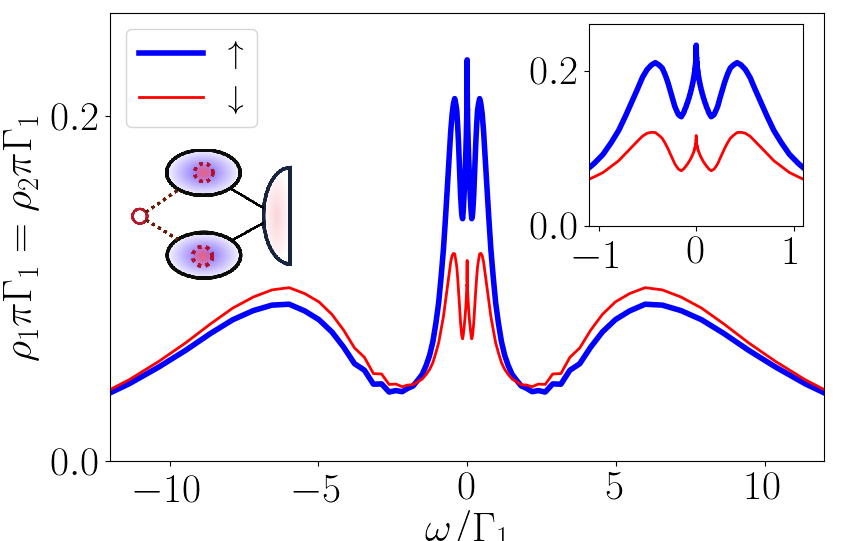
\includegraphics[scale=0.4]{Graficos/NRG-t1=t2.png}
		\caption{  \label{fig:NRG_Majorana} Density of states of both dots in the symmetric coupling without gate voltages between the Majorana and the interacting DQD. Bold blue lines: Spin-$\up$ DOS. Thin red lines: Spin-$\dw$ DOS. Inset: Low-energy DOS.
		}
		\end{center}
		\end{figure}
    %-----------E N D  F I G U R E  6 ------



 %-----------F I G U R E  7 ------
\begin{figure}[bt]
\begin{center}
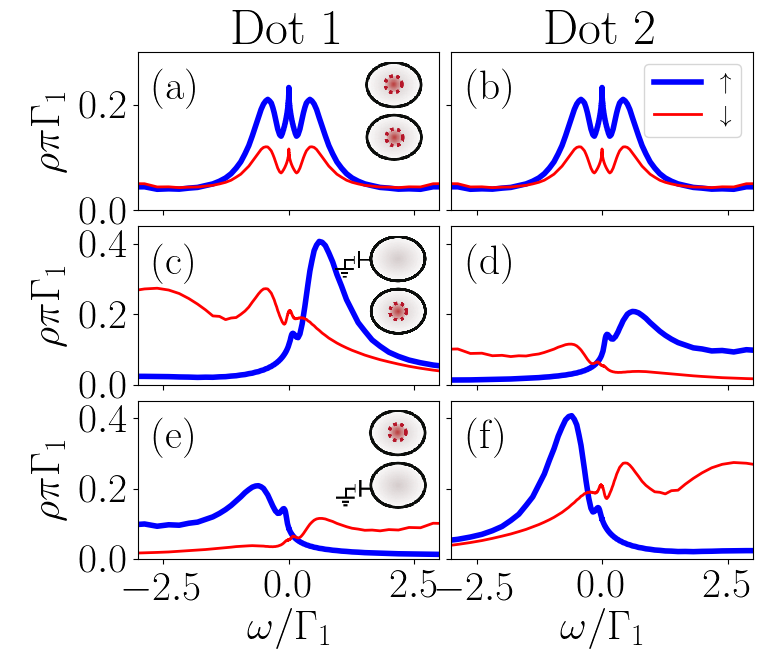
\includegraphics[scale=0.45]{Graficos/Nt1=t2.png}
\caption{ \label{fig:Nt1=t2} The same as in FIG.\ref{fig:t1=t2} for the  interacting DOS in the symmetric coupling setup (Fig.\ref{fig:MajoranaModels}.
}
%
\end{center}
\end{figure}
%-----------E N D  F I G U R E  7 ------


 %-----------F I G U R E  4 ------
\begin{figure}[bt]
\begin{center}
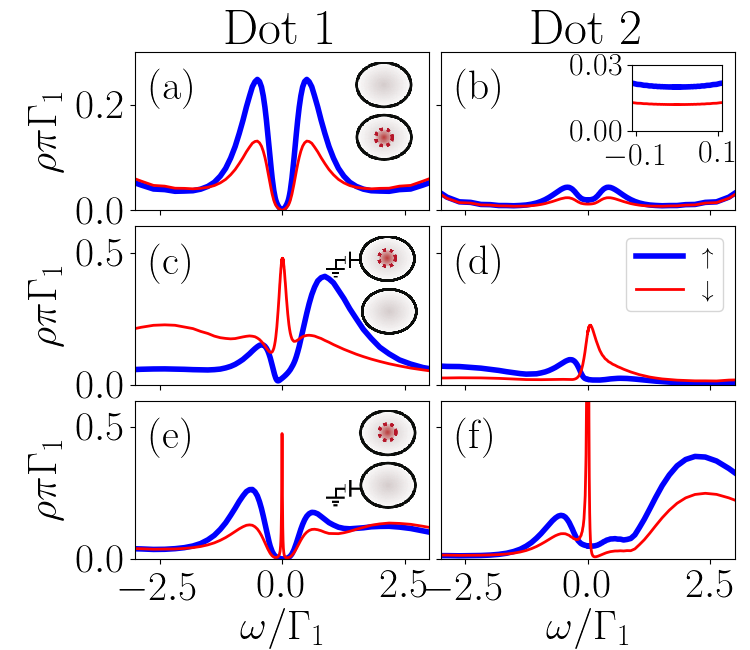
\includegraphics[scale=0.45]{Graficos/b)Nt1>0.png}
\caption{  \label{fig:Nt1>0} The same as in FIG.\ref{fig:t1=t2} for the  interacting DOS of the setup in Fig.\ref{fig:MajoranaModels}(b). Inset in b): Low-energy DOS. 
}
%
\end{center}
\end{figure}
%-----------E N D  F I G U R E  4 ------




    

    Now we consider a Coulomb repulsion energy of $U = 17\Gamma_1$ in both dots. The factor $ \frac{U_i}{2}(\sum_{\sigma} \hat{n}_{i\sigma}-1)^{2}$ in \eqref{eq:H_DQD} favors states with an odd number of electrons (and holes). In addition, particle-hole equilibrium is now achieved when $\left(\epsilon_{di}+\frac{U_i}{2}\right)\hat{n}_{i\sigma}$.  Any induced gate voltage must be considered as a shifting from this equilibrium point. FIG\ref{fig:NRG_Majorana} shows the DOS at both QDs for the symmetric coupling configuration \ref{fig:MajoranaModels}. The two peaks appearing at around $8.6\Gamma_1 = \frac{U_i}{2}$ represent the two energy levels spaced by the Coulomb repulsion factor $U$. The central spin-$\up$ peak is a consequence of the Kondo effect, \cite{hewson_kondo_1997,wilson_renormalization_1975}  while the two satellite peaks observed in the inset  are the result of the  RKKY indirect interaction between both dots.  \cite{ruderman_indirect_1954,kasuya_theory_1956,yosida_magnetic_1957} Moreover, the system presents a Majorana signature characterized by half spin-$\dw$ DOS at the Fermi energy $(\rho_\dw(0) = \frac{1}{2}\rho_\up(0))$  . Note, that in this case the Majorana signature coexists with the Kondo effect in the DQD as already predicted by Ruiz-Tijerina \textit{et al.} for a single dot. \cite{ruiz-tijerina_interaction_2015}

    In this part project we are interested in the physics at low energy scales $\omega \sim \Gamma_1 $ close to the Kondo and MZM temperature. At this scale we can observe simlar res results with the non-interacting results. For instance, FIG.\ref{fig:Nt1=t2} shows the NRG results for the symmetric setup in FIG.\ref{fig:MajoranaModels}(a). In agreement with the non-interacting results, both dots have type I Majorana signatures. These signatures can be manipulated by tuning one of the dot's gate voltage to induce the MZM to leak into the other dot. The DOS at figures FIG.\ref{fig:Nt1=t2}(d)(e) shows a type I Majorana signature with $\rho_\dw(0) \approx \frac{1}{2}\rho_\up(0))$. We observed that this Majorana signature is stable for adjustments of energies bellow the $6\Gamma_1$. At larger gate voltages the signal is  destroyed.

    %Poisoning.

    In the second setup FIG.\ref{fig:MajoranaModels}(b), the NRG results in  FIG.\ref{fig:Nt1>0} exhibit Majorana signatures similar to the non-interacting case. In the first row, the Majorana signature is destroyed by quantum interference while the second dot presents a type I Majorana signature as can be observed in the inset of the second dot. The first difference occurs when the gate voltage is switch on the first dot. This time the Majorana mode jumps onto the first dot which presents a type I Majorana signature . If the voltages is switched on the second dot, a type 2 Majorana signature appears a very low energies in dot 1. 
    
  %-----------F I G U R E  5 ------
\begin{figure}[bt]
\begin{center}
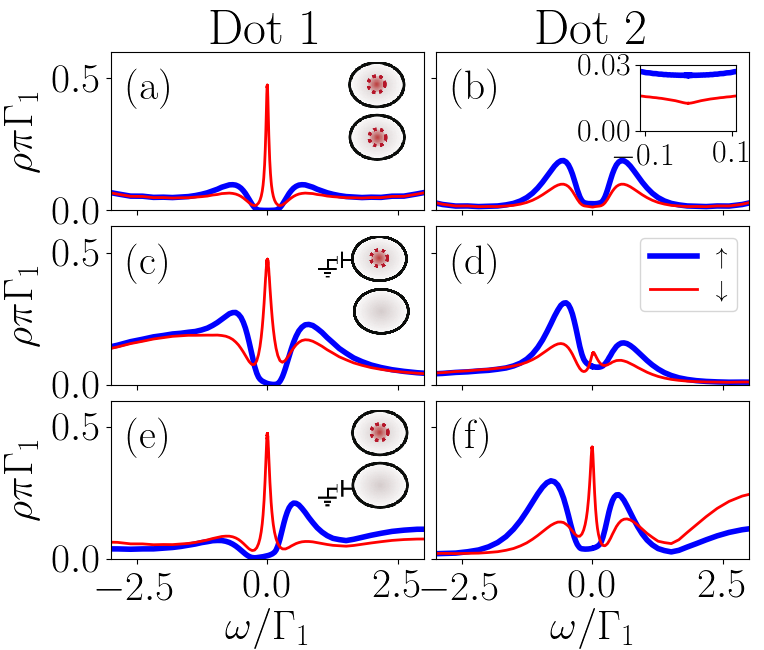
\includegraphics[scale=0.45]{Graficos/b)Nt2>0.png}
\caption{  \label{fig:Nt2>0} The same as in FIG.\ref{fig:t1=t2} for the interacting DOS of the set up in Fig.\ref{fig:MajoranaModels}(c) . Inset in b): Low-energy DOS. 
}
%

\end{center}
\end{figure}
%-----------E N D  F I G U R E  5 ------

    Finally, FIG.\ref{fig:Nt2>0} show the NRG results for the last configuration FIG.\ref{fig:MajoranaModels}(c). Surprisingly, the indirectly attached MZM exhibits a robust type II Majorana signature in the first dot over a destroyed Kondo peak. This signature is stable under the gate voltage tuning. In addition, only the first in the particle hole symmetric case the second dot presents a type II Majorana signature (Inset FIG.\ref{fig:Nt2>0}(b)). The difference between this model and the other that leads to a stable signature in one of the dots occurs because the QD's in the (c) model are connected in series. Therefore, the Majorana mode will always prevail in the dot that is attached to the leads besides the application of gate voltages. This case is similar to the model of a single dot attached to a Majorana chain, where it is known that the Majorana signatures is not disturbed by the gate tuning. 
%---------------------------------------------------------------------------  
\section{Concluding remarks}
\label{sec:Conclusions}
Comparing the exact analytical solution in the non-interacting system and the NRG results for interacting quantum dots, we were able to characterized the displacements of the MZM inside the double quantum dot for the three setups in FIG.\ref{fig:MajoranaModels}. We observe a considerable agreement on the location of the Majorana signature between the interacting and non-interacting results:

\begin{itemize}
	\item[]FIG.\ref{fig:MajoranaModels}(a): In the symmetric coupling the MZM leaks inside both dots. For interacting dots, the Majorana signature will be distinguishable near the Kondo temperature. At this regime the system presents combined Kondo-Majorana physics . If the gate voltage of one dot is turned on the MZM is induced to tunnel only into the other dot.  
	\item[]FIG.\ref{fig:MajoranaModels}(b): In this system the spin-$\up$ zero mode at QD1 (The Kondo peak if the system is interacting) is destroyed by quantum interference with the second dot. This interference will also destroy the MZM in the first dot but a type I Majorana signature will still appear in the second dot. The Majorana mode can be induced to tunnel back into the first dot if a gate voltage is applied on the second dot. This signature is visible at very low energies (bellow $0.1\Gamma_1$) in interacting case. 
	\item[]FIG.\ref{fig:MajoranaModels}(c): An indirect type II Majorana signature is observed in the first dot. This signature is robust, specially in the interacting case, where it is present in all configurations. 

\end{itemize}

 % We observed considerable agreements between both In the symmetric coupling

\begin{acknowledgments}
The authors thank Edson Vernek for enlightening discussions.  L.G.G.V.D.S. acknowledges financial support by CNPq (grants No. 307107/2013-2 and 449148/2014-9), and FAPESP (grant No. 2016/18495-4).
\end{acknowledgments}

% \LUIS{Only ONE bib file}

%---------------------- Apendix A------------------------


%-----------------------------------------------------------

%\bibliographystyle{unsrtnat}
%\addcontentsline{toc}{section}{\textbf{References}}
\bibliography{Majorana_DQD.bib}



 \appendix

 
 \section{Computation of the Green Function \label{sec:Appendix_alg}}
 In Zubarev's fermionic ballistic transport approach \cite{zubarev_double-time_1960} the green function associated to two operators $A(t)$ , $B(t)$ is defined as that Fourier transform of the time-ordered anti-commutator of $A$ and $B$
\begin{equation}
  \Green{A,B}= \mathcal{F}\left\{ \mathcal{T}\left[\left\{ A(t),B(t')\right\} \right]\right\} \left(\omega\right).
  \label{eq:greenFunction}
\end{equation}

The Fourier transform of Schrodinger evolution leads to the the transport equations 
\begin{equation}
    \omega\Green{A,B}=\delta_{A^{\dagger},B}+\Green{\left[A,H\right],B}.
    \label{eq:Transport}
\end{equation}
\noindent Applying this expression to Hamiltonian \eqref{eq:Model} replacing $A$ and $B$ by the creation and annihilation operators $d\dagger_i, f^\dagger, d_i,f ,c_k,c\dagger_k$ we obtain a linear transport system. To simplify the complexity of the equations we fix $B = d^\dagger_{1\dw}$. In addition note that if we replace $A$ by $f_\dw$ and $f^\dagger_\dw$ \ref{eq:Transport} becomes
\begin{align}
        \left(\omega-\epsilon_{M}\right)\Green{f_{\downarrow},d_{1\downarrow}^{\dagger}}&=\frac{t}{\sqrt{2}}\left(\Green{d_{1\downarrow},d_{1\downarrow}^{\dagger}}-\Green{d_{1\downarrow}^{\dagger},d_{1\downarrow}^{\dagger}}\right) \\
    \left(\omega+\epsilon_{M}\right)\Green{f_{\downarrow}^{\dagger},d_{1\downarrow}^{\dagger}}&=\frac{t}{\sqrt{2}}\left(\Green{d_{1\downarrow},d_{1\downarrow}^{\dagger}}-\Green{d_{1\downarrow}^{\dagger},d_{1\downarrow}^{\dagger}}\right).
\end{align}
\noindent This allows us to take $\Green{f_{\downarrow}^{\dagger},d_{1\downarrow}^{\dagger}} = \frac{\omega + \epsilon}{\omega -\epsilon}\Green{f_{\downarrow}^{\dagger},d_{1\downarrow}^{\dagger}} $. Hence, we can eliminate $\Green{f_{\downarrow}^{\dagger},d_{1\downarrow}^{\dagger}} $ from the equations even before we start Gauss-Jordan process.

Writing the other equations  we obtain the  linear system of the form
\begin{equation}
    \mathcal{T} \vec{G}_{d^\dagger_1} = \hat{e_1},
\end{equation}

\noindent where $\mathcal{T}$ is the transport matrix 
\begin{equation}
\left[\begin{array}{ccccccc}
\omega-\epsilon_{1} & -V_{1}^{*} & -t_{dots} & \frac{-t_{1}}{\sqrt{2}} & 0 & 0 & 0\\
-V_{1} & \omega-\epsilon_{k} & -V_{2} & 0 & 0 & 0 & 0\\
-t_{dots}^{*} & -V_{2}^{*} & \omega-\epsilon_{2} & \frac{-t_{2}}{\sqrt{2}} & 0 & 0 & 0\\
\frac{-\sqrt{2}t_{1}^{*}}{\omega+\epsilon_{M}} & 0 & \frac{-\sqrt{2}t_{2}^{*}}{\omega+\epsilon_{M}} & \omega-\epsilon_{M} & \frac{\sqrt{2}t_{2}^{*}}{\omega+\epsilon_{M}} & 0 & \frac{\sqrt{2}t_{1}^{*}}{\omega+\epsilon_{M}}\\
0 & 0 & 0 & \frac{t_{2}}{\sqrt{2}} & \omega+\epsilon_{2} & V_{2}^{*} & t_{dots}^{*}\\
0 & 0 & 0 & 0 & V_{2} & \omega+\epsilon_{k} & V_{1}\\
0 & 0 & 0 & \frac{t_{1}}{\sqrt{2}} & t_{dots} & V_{1}^{*} & \omega+\epsilon_{1}
\end{array}\right],
\label{eq:TransportMatrix}
\end{equation}
 \noindent $\vec{G}_{d^\dagger_1}$  is the column vector
%  wit indices
%  $\Green{d_{\mathbf{1\downarrow}},d_{1\downarrow}^{\dagger}},\Green{c_{k\downarrow},d_{1\downarrow}^{\dagger}},\Green{d_{2\downarrow},d_{1\downarrow}^{\dagger}}$
% %  $ \Green{d_{\mathbf{1\downarrow}},d_{1\downarrow}^{\dagger}},\Green{c_{k\downarrow},d_{1\downarrow}^{\dagger}},\Green{d_{2\downarrow},d_{1\downarrow}^{\dagger}},\Green{f_{\downarrow}$
 
 \begin{align*}
    [ \Green{d_{\mathbf{1\downarrow}},d_{1\downarrow}^{\dagger}},&\Green{c_{k\downarrow},d_{1\downarrow}^{\dagger}},\Green{d_{2\downarrow},d_{1\downarrow}^{\dagger}},\Green{f_{\downarrow},  d_{1\downarrow}^{\dagger}}, \\ & \Green{d_{2\downarrow}^{\dagger},d_{1\downarrow}^{\dagger}},\Green{c_{k\downarrow}^{\dagger},d_{1\downarrow}^{\dagger}},\Green{d_{1\downarrow}^{\dagger},d_{1\downarrow}^{\dagger}} ]^T
 \end{align*}
and $\hat{e_1}$ is the vector with entries  $\hat{e}_{1_n} =\delta_{1n}$. 

The graph associated to this matrix is the one in FIG.\ref{fig:Transport}. The energies inside each vertex are given by subtracting the corresponding diagonal term from $\omega$ . The couplings are just the negative of the off-diagonal terms. 

\subsection{The double quantum dot}


% %-----------F I G U R E  Graph ------
        \begin{figure}[t]
        \begin{center}
        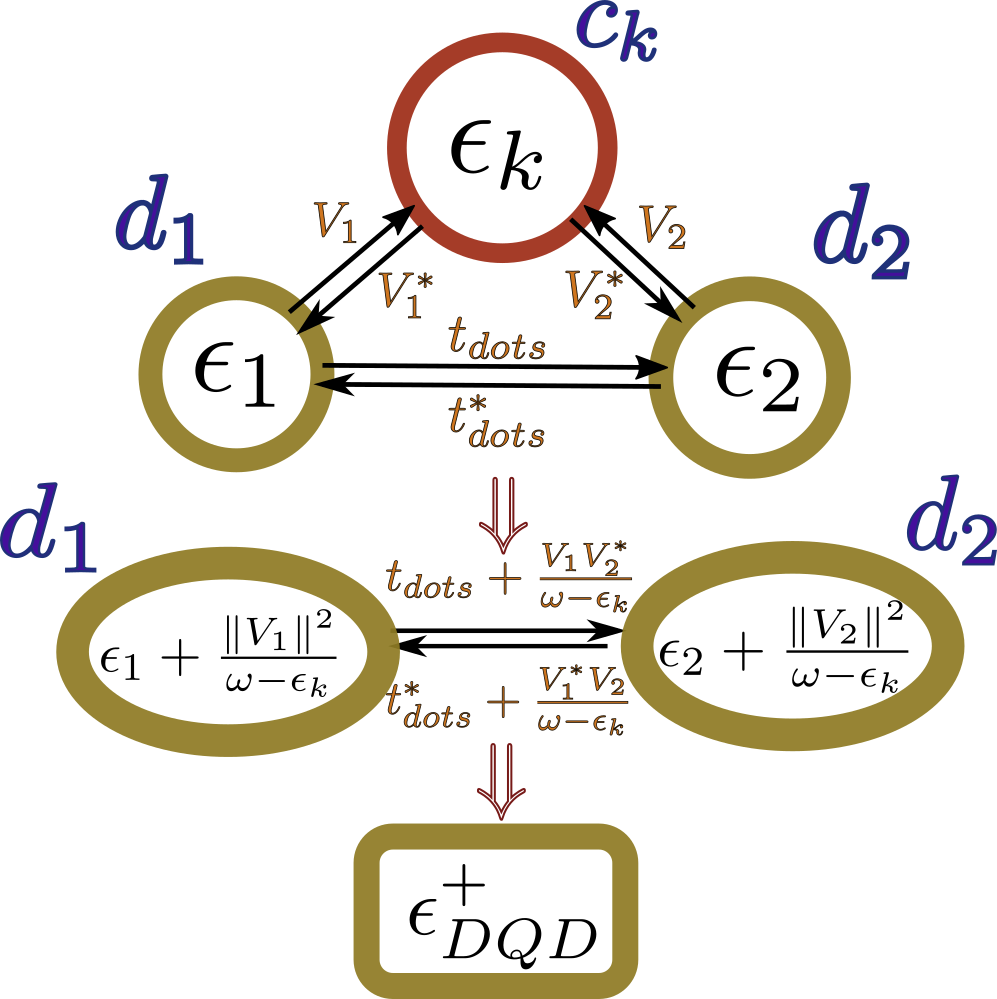
\includegraphics[scale=0.25]{Graficos/Graph_DQD-Pro.png}
        \caption{ 
        }
        %
        \label{fig:GraphsDQD}
        \end{center}
        \end{figure}
%-----------E N D  F I G U R E  1 ------




To explain the process of Gaussian elimination we will obtain the green function for the case without Majorana fermion $(t_1= t_2=0)$.  The transport matrix for this system is 
\begin{equation}
        \left[\begin{array}{ccc}
    \omega-\epsilon_{1} & -V_{1} & -t_{dots}\\
    -V_{1}^{*} & \omega-\epsilon_{k} & -V_{2}\\
    -t_{dots}^{*} & -V_{2}^{*} & \omega-\epsilon_{2}
    \end{array}\right]. \label{eq:DQDMatrix}
\end{equation}

\noindent The graph associated to this matrix can be observed in FIG\ref{fig:GraphsDQD}.a). To eliminate the vertex $c_k$ we just need to subtract from \eqref{eq:DQDMatrix} the rank-$1$ matrix that cancels the row and the column corresponding to $c_k$. This matrix is 
\begin{equation}
        \left[\begin{array}{ccc}
    \frac{V_{1}^{*}V_{1}}{\omega-\epsilon_{k}} & -V_{1}^{*} & \frac{V_{2}V_{1}^{*}}{\omega-\epsilon_{k}}\\
    -V_{1} & \omega-\epsilon_{k} & -V_{2}\\
    \frac{V_{2}^{*}V_{1}}{\omega-\epsilon_{k}} & -V_{2}^{*} & \frac{V_{2}^{*}V_{2}}{\omega-\epsilon_{k}}
    \end{array}\right]. \label{eq:rank1}
\end{equation}
The result of \eqref{eq:DQDMatrix} -  \eqref{eq:rank1} is 



%-----------F I G U R E  2 ------

    \begin{figure}[t]
    \begin{center}
    \centering
     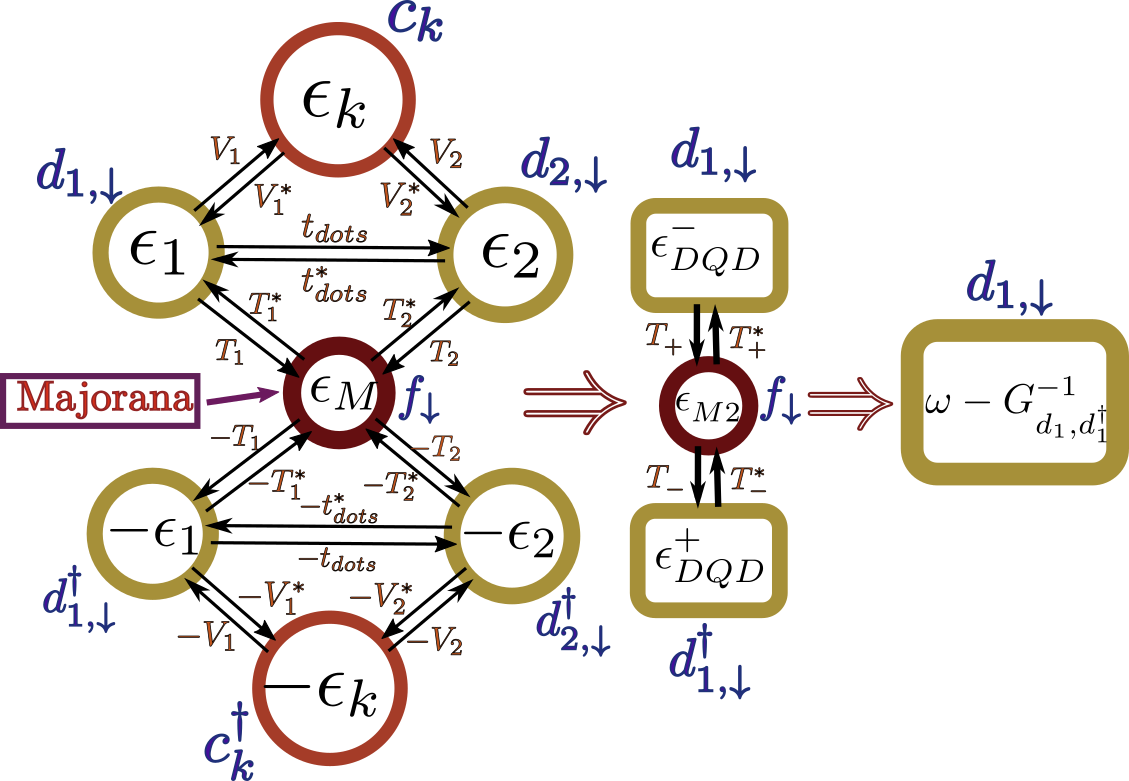
\includegraphics[scale=0.29]{Graficos/Graphs-DQD-M-Pro.png}
    % 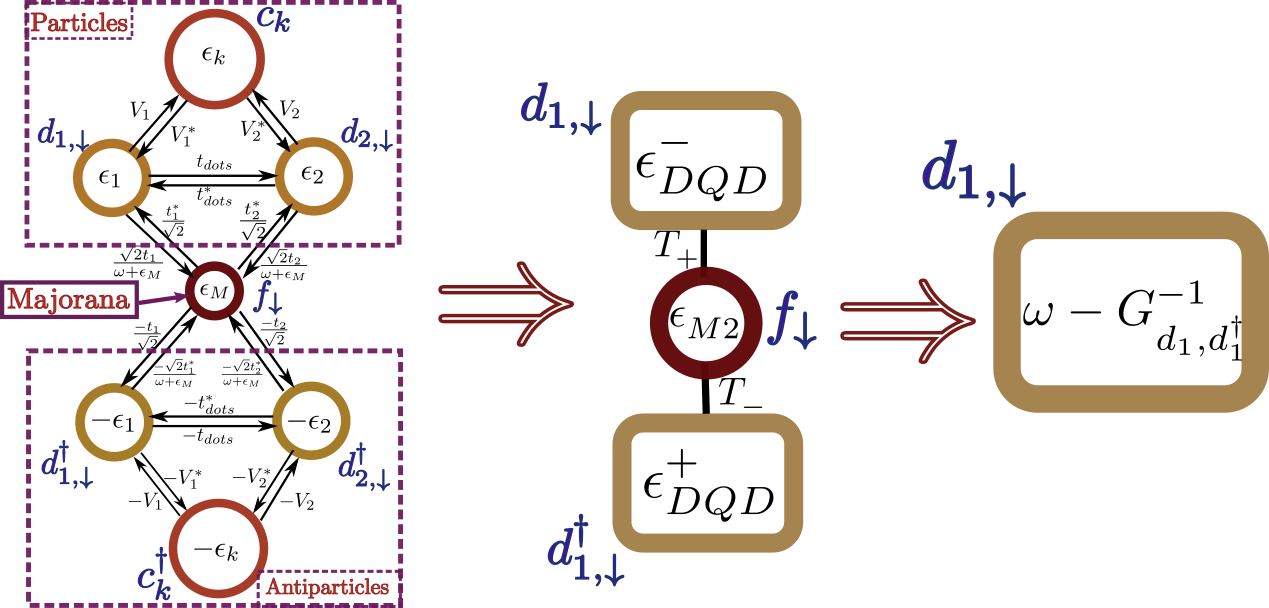
\includegraphics[scale=0.25]{Graficos/graphContractions.png}
    \caption{ Transport flow in a DQD Majorana system.   \label{fig:Transport}
    }
    %
    
    \end{center}
    \end{figure}

%-----------E N D  F I G U R E  2 ------




\begin{equation}
        \left[\begin{array}{ccc}
    \omega-\epsilon_{1}-\frac{V_{1}^{*}V_{1}}{\omega-\epsilon_{k}} & 0 & -t_{dots}-\frac{V_{2}V_{1}^{*}}{\omega-\epsilon_{k}}\\
    0 & 0 & 0\\
    -t_{dots}^{*}-\frac{V_{2}^{*}V_{1}}{\omega-\epsilon_{k}} & 0 & \omega-\epsilon_{2}-\frac{V_{2}V_{1}^{*}}{\omega-\epsilon_{k}}
    \end{array}\right]
\end{equation}
\noindent which is depicted by the graphs in FIG.\ref{fig:GraphsDQD}.b). The next step is to pop-out the vertex $d_2$ following the same procedure. At the end, the energy inside the vertex $d_1$ will be
\begin{equation}
    \epsilon^+_{DQD}=\epsilon_{1}+\sum_{\mathbf{k}}\frac{V_{1}V_{1}^{*}}{\omega-\epsilon_{\mathbf{k}}}+\frac{\left\Vert t_{dots}+\sum_{\mathbf{k}}\frac{V_{1}V_{2}^{*}}{\omega-\epsilon_{\mathbf{k}}}\right\Vert ^{2}}{\omega-\epsilon_{2}-\sum_{\mathbf{k}}\frac{V_{2}V_{2}^{*}}{\omega-\epsilon_{\mathbf{k}}}} \label{eq:EnDQD}
\end{equation}
and the green function of $\Green{d_1d^\dagger_1}$ in a DQD will be given by $\frac{1}{\omega -  \epsilon_{DQD}}$ (see FIG.\ref{fig:GraphsDQD}.c)).

\subsection{Solution of the transport equations}

The previous procedure can be generalized into the following algorithm:

\begin{enumerate}
    \item Computing the transport equations with the second term fixed in the creation operator of the dot.
     \item  Setting up the  graph associated to the transport system.
    \item Popping out the vertexes of the graph. Each popping process carries the following steps.
    \begin{enumerate}
        \item Computing the extra-terms in the energies and couplings based on the walks passing through the popped vertex.
        \item Eliminating this vertex from the graph. 
        \item Iterating till there is only one  vertex.
        \end{enumerate}
    \item The energy in the remaining vertex $d$ is $\epsilon_d = \frac{1}{\omega -\Green{d,d\dagger}}$ .
\end{enumerate}
  


Following these steps it is possible to solve the general case.  We start with the graph in FIG.\ref{fig:Transport} and we pop out the vertexes $c_k,c^\dagger_k, d_{2,\dw}$ and $ d^\dagger_{2,\dw}$ in that order. The energies associated to $d_{1,\dw}$ and $d^\dagger_{1,\dw}$ will be similar to \eqref{eq:EnDQD} giving 
\begin{equation}
    \epsilon_{DQD}^{\pm}=\pm\epsilon_{1}+\sum_{\mathbf{k}}\frac{V_{1}V_{1}^{*}}{\omega-\epsilon_{\mathbf{k}}}+\frac{\left\Vert \pm t_{dots}+\sum_{\mathbf{k}}\frac{V_{1}V_{2}^{*}}{\omega-\epsilon_{\mathbf{k}}}\right\Vert ^{2}}{\omega\pm\epsilon_{2}-\sum_{\mathbf{k}}\frac{V_{2}V_{2}^{*}}{\omega-\epsilon_{\mathbf{k}}}}. \label{eq:epDQD}
\end{equation}
\noindent There is also a correction in the couplings between the Majorana mode and $d_{1,\dw}$, $d^\dagger_{1,\dw}$ given by 

\begin{equation}
    T_{\pm}=\pm t_{1}\pm t_{2}\frac{\left(\pm t_{dots}+\sum_{\mathbf{k}}\frac{V_{1}V_{2}^{*}}{\omega-\epsilon_{\mathbf{k}}}\right)}{\omega\pm\epsilon_{2}\pm\sum_{\mathbf{k}}\frac{V_{2}V_{2}^{*}}{\omega-\epsilon_{\mathbf{k}}}}. \label{eq:T+-}
\end{equation}

Finally since the Majorana is in contact with dot $2$, there is an extra-term appearing in the  Majorana energy given by 
\begin{equation}
    \epsilon_{M2}=\omega-\epsilon_{M}-\frac{\frac{\omega}{\omega+\epsilon_{M}}\left\Vert t_{2}\right\Vert ^{2} } {\omega-\epsilon_{2}-\sum_{\mathbf{k}}\frac{V_{2}V_{2}^{*}}{\omega-\epsilon_{\mathbf{k}}}}-\frac{\frac{\omega}{\omega+\epsilon_{M}}\left\Vert t_{2}\right\Vert ^{2}}{\omega+\epsilon_{2}-\sum_{\mathbf{k}}\frac{V_{2}V_{2}^{*}}{\omega+\epsilon_{\mathbf{k}}}}. \label{eq:M2_append}
\end{equation}
With all the terms of the graph in FIG.\ref{fig:Transport}.b) computed, it only remains to pop out vertexes $d^\dagger_1$ and $f_\dw$ in that order to obtain the result in equation \eqref{eq:Green_NonInteracting}. 


\begin{equation}
    G_{{d_{1\downarrow},d_{1\downarrow}^{\dagger}}}\left(\omega\right)=\frac{1}{\omega-\epsilon_{DQD}^{+}-\frac{\left\Vert T_{+}\right\Vert ^{2}}{\omega-\epsilon_{M2}-\frac{\left\Vert T_{-}\right\Vert ^{2}}{\epsilon_{DQD}^{-}}}}.
     \label{eq:2Green_NonInteracting}
\end{equation}

\noindent From this analytical expression we can compute rapidly dynamical quantities such as the density of states in the non-interacting regime. Despite the difference this became a useful idea to predict interesting parameters for NRG simulation. Since the NRG code  code takes about an hour to simulate each set of parameters in the Majorana-DQD mode, and even more if additional implementations are necessary, \ref{eq:2Green_NonInteracting} became an important tool to improve our results. 






%---------------------------------------------------------------------------
 



% %-----------F I G U R E  Graph ------
% \begin{figure}[bt]
% \begin{center}
% 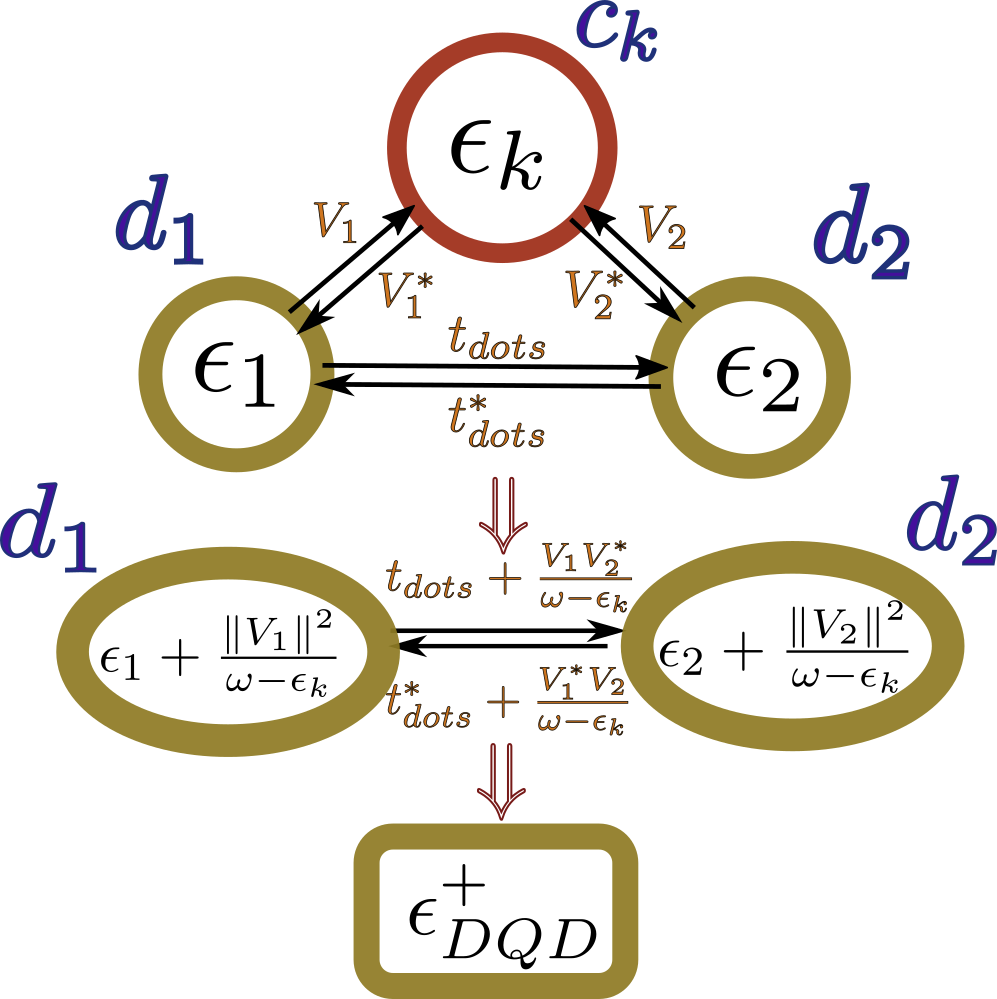
\includegraphics[scale=0.2]{Graficos/Graph_DQD-Pro.png}
% \caption{ 
% }
% %
% \label{fig:GenModel}
% \end{center}
% \end{figure}
% %-----------E N D  F I G U R E  1 ------





\end{document}










% To simplify the solution of this system we used a graph linear algorithm  that speeds-up the process of Gauss-Jordan elimination. \cite{spielman_algorithms_2010} Starting with the flow graph at FIG.\ref{fig:Transport} (a), the algorithm successively "pops"  the vertexes till only one vertex remains in the  graph. Popping a vertex must be understood as the Gaussian elimination of the line and the column in the transport matrix containing that vertex (Appendix \ref{sec:Appendix_alg}). This modifies the energies of the vertexes and the coupling parameters. Changing the order of elimination of the vertexes could lead to different equivalent representations of the final polynomial. Finding a suitable elimination order could significantly reduce the complexity of the solution. \cite{spielman_algorithms_2010}  


% The flow graph in FIG.\ref{fig:Transport} depicts the linear map associated to the transport in an hybrid Majorana-DQD system  \eqref{eq:TransportMatrix} . The energies of each operator are located at the center of the vertexes while the vertex couplings represent the off-diagonal terms.  The Majorana mode connects two regions of the graph, both of them representing a DQD. The upper DQD is conformed by annihilation operators while the lower one is formed by creation operators. The couplings in the lower part are the  upper parameters multiplied by $-1$. 

% to study the non-interacting system $U=0$. Without 






% To study the non-interacting case $(U=0)$, we use Zubarev's ballistic transport approach \cite{zubarev_double-time_1960} to compute the Green functions associated to both quantum dot operators $(\Green{d_1d^\dagger_1},\Green{d_2d^\dagger_2})$. The detailed procedure is included in Appendix \ref{sec:Appendix_alg}. The transport equations define a linear system where the Hamiltonian parameters $(t_1,t_2,\epsilon_1 \ldots)$ and the energy $\omega$ are taken as fix variables. The flow graph in FIG.\ref{fig:Transport} depicts the linear map associated to the transport in an hybrid Majorana-DQD system  \eqref{eq:TransportMatrix} . The energies of each operator are located at the center of the vertexes while the vertex couplings represent the off-diagonal terms.  The Majorana mode connects two regions of the graph, both of them representing a DQD. The upper DQD is conformed by annihilation operators while the lower one is formed by creation operators. The couplings in the lower part are the  upper parameters multiplied by $-1$. 

% To simplify the solution of this system we used a graph linear algorithm  that speeds-up the process of Gauss-Jordan elimination. \cite{spielman_algorithms_2010} Starting with the flow graph at FIG.\ref{fig:Transport} (a), the algorithm successively "pops"  the vertexes till only one vertex remains in the  graph. Popping a vertex must be understood as the Gaussian elimination of the line and the column in the transport matrix containing that vertex (Appendix \ref{sec:Appendix_alg}). This modifies the energies of the vertexes and the coupling parameters. Changing the order of elimination of the vertexes could lead to different equivalent representations of the final polynomial. Finding a suitable elimination order could significantly reduce the complexity of the solution. \cite{spielman_algorithms_2010}  


% This graph-linear solver algorithm turns out to be particularly good for Majorana systems  since the Majorana fermion is a natural cutting point that divides the graph in two sections. This allows us to exploit the graph structure to simplify the solution of the system  by selecting a suitable order of vertex-elimination . Fig.\ref{fig:Transport} depicts this process. In the first step (a) to (b), we pop consecutively the vertexes $c_{k,\dw},c_{k,\dw}^\dagger , d_{2,\dw} , d^\dagger_{2,\dw}$. The new parameters $\epsilon^{\pm}_{DQD}$ , $M_2$ and $T_\pm$ (See Appendix \ref{sec:Appendix_alg}) are functions of $\epsilon_1 , \epsilon_2 , t_1,t_2$, etc . These functions gather the transport information  through the popped vertexes . The next step is to pop vertexes $d_{1,\dw}^\dagger$ and $f_{\dw}$, which condensed the transport information of the whole system into the remaining vertex $d_{1,\dw}$ . As shown in Appendix \ref{sec:Appendix_alg} the energy of vertex $d_{1,\dw}$ is $\omega - \Green{d_1\dw d^\dagger_1\dw } $, hence giving a very compact expression for the Green function

% % This process can be observed graphically in figure \ref{fig:Transport}. In the first step (a) to (b), we pop-out consecutively the vertexes $c_{k,\dw},c_{k,\dw}^\dagger , d_{2,\dw} , d^\dagger_{2,\dw}$. The transport information through these vertexes is   in the operators  $d_{1,\dw}$, $d_{1,\dw}^\dagger$ and $f_\dw$, such that the energies $\epsilon^{\pm}_{DQD}$ accumulate the information of both double quantum dots while the couplings are modified to $T_\pm$. The last step is to pop-out vertexes $d_{1,\dw}^\dagger$ and $f_{\dw}$. At the end of the whole process the energy of the remaining vertex $d_{1,\dw}$ contains the green function $\Green{d_1\dw d^\dagger_1\dw } $ giving this very compact expression
% \begin{equation}
%     G_{{d_{1\downarrow},d_{1\downarrow}^{\dagger}}}\left(\omega\right)=\frac{1}{\omega-\epsilon_{DQD}^{+}-\frac{\left\Vert T_{+}\right\Vert ^{2}}{\omega-\epsilon_{M2}-\frac{\left\Vert T_{-}\right\Vert ^{2}}{\epsilon_{DQD}^{-}}}}.
%     \label{eq:Green_NonInteracting}
% \end{equation}


% % Note also that the spin-$\up$ green functions  can be obtained by replacing the Majorana couplings $t_1,t_2 = 0$.
% The final result will depend on the broadening parameter of QD $i$ with the lead $(\Gamma_i)$. This broadening satisfies the equation

% \begin{equation}
%    -i\Gamma_i = \lim_{s\rightarrow 0} \sum_{\boldsymbol{k}}\frac{V_{i}^{*}V_{i}}{\omega+ is -\epsilon_{\boldsymbol{k}}}.
% \end{equation}

% By convention we will take $\Gamma_1$ as the energy unit for the rest of the project. Finally we compute the DOS 


% \begin{equation}
%     \rho_{1\sigma}(\omega)=-\frac{1}{\pi} \textrm{Im} \left[G_{d_{1\sigma},d_{1\sigma}^\dagger}(\omega))\right].
%     \label{eq:Density of States}
% \end{equation}
% Similar results can be obtain for the DOS of the second $\rho_{2\sigma}$ . Comparing these results for both dots at the Fermi energy we will be able to determine which dot exhibits a Majorana signature.


% % The green functions $(\Green{d_1d^\dagger_1},\Green{d_2d^\dagger_2})$  obtained through Gauss-Jordan elimination constitute fractional polynomial with more than $300$ independent linear components. To provide a tractable decomposition of this polynomial we used a graph theory-inspired linear algorithm that emulates a Laplacian linear solver . Although this Hamiltonian is not Laplacian,  this method still provides a shortcut to Gauss-Jordan elimination by taking advantage of the minimal cuttings in the graph. As a matter of fact , this graph approach is especially good for Majorana systems  since the Majorana fermion is a natural cutting point that divides two sections of the graph.  
% % In addition the graph contraction facilitates a legible representation of the fractional polynomial.
% % The solution of this problem can be achieved through 
% % In a system without Majorana fermions these two regions are disconnected. The new physical   











































    % orana mode is connected to the first dot, this interference will destroy the majorana signature in the first dot. Interestingly, it is possible to observe a clear majorana signature in the second dot caracterized by a half central peak in the spin-$dw$ DOS. While turning on the first dot gate volge seems to destroy this ajorana signature, tuning the second dots gate voltage returns the majorana signature to the first dot. 
% =======
%      The density of states for the set-ups in column $1$ (FIG.\ref{fig:MajoranaModels}) is shown in Figure \ref{fig:t1=t2}. Since the model is non-interacting, spin-$\up$ and spin-$\dw$ models are independent. The spin-$\dw$ DOS (dashed line) shows the effects caused by the majorana mode in comparison with the spin-$\up$  results (solid line). In the particle hole symmetric case the DOS is equal in both dots. Note that that the spin-$\dw$ DOS is the half of the spin-$DOS$ at the fermi energy $\rho_\dw(0) = \rho_\up(0)$. This is a Majorana signature similar to the one observed in the single dot case \cite{liu_detecting_2011}. Hence, the majorana tunnels inside both dots. When a possitive or negative gate voltage is induced in one of the dots,  the Majorana mode is induced to leave that dot. As consequence the majorana signature will only appear in the other dot. 
     
%     If the second dot is not directly connected to the lead some interesting results appear. In this set-up the induced tunneling between both dots generated a path difference that destroys the central peak (See FIG\ref{fig:Interference} spin-$\up$ line). If the Majorana mode is connected to the first dot, this interference will destroy the majorana signature in the first dot. Interestingly, it is possible to observe a clear majorana signature in the second dot caracterized by a half central peak in the spin-$dw$ DOS. While turning on the first dot gate volge seems to destroy this majorana signature, tuning the second dots gate voltage returns the majorana signature to the first dot. 
% >>>>>>> 4c82b0d0ee9129153656d93fa0c73cf179fcaaea
    





% \section{Atomic limit: Change of basis}
% Returning to Hamiltonian \eqref{eq:AtomicHam} the change of basis is given by 
% \[
%   d_{+ , \sigma} = \frac{1}{\sqrt{2}} (d_{1\sigma} +d_{2\sigma}) \ , \ 
%   d_{- , \sigma} = \frac{1}{\sqrt{2}} (d_{1\sigma} -d_{2\sigma}).
% \]

% These new operators satisfy the fermionic anti-commutation relations 
%  \[ \{d_{\pm , \sigma}, d^\dagger_{\pm , \sigma}\} = 1 , \{ d_{\pm , \sigma}, d^\dagger_{\mp , \sigma}\} = 0,
% \]
%  so that the may be considered as fermion operators. All lineal terms in \eqref{eq:AtomicHam} are trivially adapted to the new base. The repulsion potential 
% $$\sum_{i} (\sum_{\sigma} d_{i \sigma}^{\dagger}d_{i \sigma}-1)^{2} = (\sum_{\sigma} d_{1 \sigma}^{\dagger}d_{1 \sigma}-1)^{2} + (\sum_{\sigma} d_{2 \sigma}^{\dagger}d_{2 \sigma}-1)^{2} . $$ 
% gives rise to a non-trivial interaction between the new states. To find this interaction we define the particle number operator  
% \[\hat{n}_{i,\sigma}:= d^\dagger_{i,\sigma}d_{i,\sigma}.\] 

% So that 
% \begin{align}
% \hat{n}_{1,\sigma}= & \frac{1}{2} \left( \hat{n}_{+,\sigma} + \hat{n}_{-,\sigma} + d^\dagger_{+,\sigma}d_{-,\sigma} + d^\dagger_{-,\sigma}d_{+,\sigma} \right) \\
% = & \frac{1}{2} \left( \hat{N}_\sigma + \hat{E}_\sigma \right),
% \end{align}
% with $\hat{N}_\sigma = \hat{n}_{+,\sigma} + \hat{n}_{-,\sigma}$ and $\hat{E}_\sigma = d^\dagger_{+,\sigma}d_{-,\sigma} + d^\dagger_{-,\sigma}d_{+,\sigma}. $ Similarly 

% \[\hat{n}_{2,\sigma}= \frac{1}{2} \left( \hat{N}_\sigma - \hat{E}_\sigma \right).  \]
% Hence 
% \begin{align}
% \sum_{i} (\sum_{\sigma} d_{i \sigma}^{\dagger}d_{i \sigma}-1)^{2} = & \left(\frac{\hat{N} +\hat{E}}{2}-1 \right) ^{2} + \left( \frac{\hat{N} -\hat{E}}{2}-1 \right)^{2} \\
%  = & \frac{\left( \hat{N}-2 \right)^2- \hat{E}^2}{2},
% \end{align}

% with $\hat{N}_\sigma=\sum_\sigma \hat{N}_\sigma $ , $\hat{E}=\sum_\sigma \hat{E}_\sigma $. Note that opeator $\hat{N}$ represents the total occupation number inside both dots. If this occupation is different than $2$ there is an imbalance between particles and dots that is punished by this term. The term $E^2$ is much more interesting since this one is the responsible for the emergence of satellite peaks in the DOS. To understand what it makes it is simple to observe its results when applied to a based ordered by $\vert + , - \rangle$. 
% \[ \hat{E}^2 \vert \up , 0 \rangle =  \hat{E} \vert 0 , \up \rangle = \vert \up , 0 \rangle   \] 
% \[ \hat{E}^2 \vert \up , \dw \rangle =  \hat{E} \left( \vert 0 , \up\!\dw \rangle + \vert \up\!\dw , 0 \rangle \right) = 2\vert \up , \dw \rangle - 2\vert \dw , \up \rangle  \]

% \begin{align}
% H = \sum_{\sigma}  \frac{U}{4}\left( \left( \hat{N}-2 \right)^2- \hat{E}^2 \right) + \frac{t}{\sqrt{2}} (\gamma_1 d_{+,\dw}+d^\dagger_{+,\dw}\gamma_1 )
% \label{t+}
% \end{align}




 This system is already closed which means that we don't need any other equation to find the solution. The matrix form takes the form
 \begin{equation}
\left[\begin{array}{ccc}
\omega-\epsilon_{2} & -V_{2} & -t_{dots}\\
-V_{2}^{*} & \omega-\epsilon_{k} & -V_{1}\\
-t_{dots}^{*} & -V_{1}^{*} & \omega-\epsilon_{1}
\end{array}\right]\left[\begin{array}{c}
\Green{c_{\mathbf{k}},d_{1}^{\dagger}}\\
\Green{d_2,d_{1}^{\dagger}}\\
\Green{d_{1},d_{1}^{\dagger}}
\end{array}\right]=\left[\begin{array}{c}
0\\
0\\
1
\end{array}\right]
\label{eq:MatrixDQD}
 \end{equation}
 
\noindent By convenience we changed the order of the rows in the matrix. Although this matrix is not Laplacian, the procedure in \cite{spielman10} can still be applied with the downside of loosing some of the speed-up advantages of the algorithm. Still, some advantages of graphs are preserved. From these we point out  the possibility of taking taking minimal cuttings and the relation between these graphs and random walks in the graph. Both advantages simplify the complexity of the solution. 
 
Now, our objective is to compute the green function  $\Green{d_{1\downarrow},d_{1\downarrow}^{\dagger}}$.   For this we take the graph $\GDQD$ associated to the matrix in \eqref{eq:MatrixDQD}. The result is observed in \ref{fig:graphDQD}.a).  The vertexes of this graph will be the operators in the first site of the of the green functions  $(d_{1\downarrow},d_{2},c_{\boldsymbol{k}}$. $d_1^\dagger)$. $d^\dagger_1$ is not included since it only appears in the second sub-index of the green functions. The edges are given by the non-diagonal sites in the matrix. In addition, an energy parameter is assigned to each vertex, according to the corresponding term in the diagonal. These energies can also be taken as edges connecting each vertex with itself. 

% \begin{figure}[t]
%     \centering
%     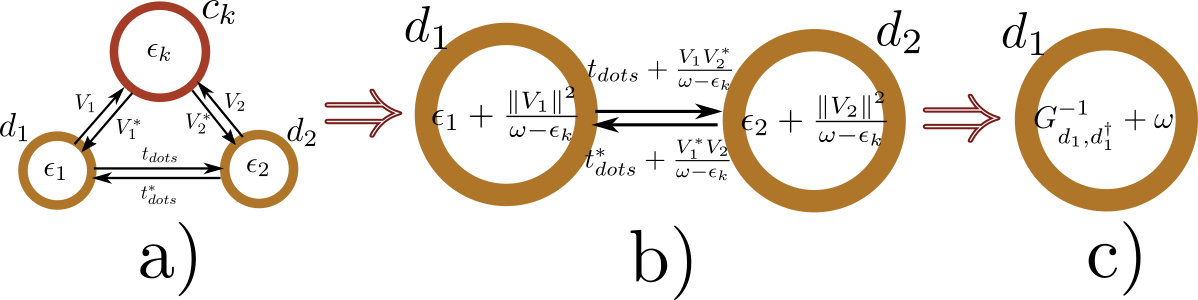
\includegraphics[scale=0.4]{IMAGES/Graphs/DQD-Pro.png}
%     \caption{ a) Graph $\GDQD$ b) After the elimination of vertex $c_k$, the energies of dots $d_1$ and $d_2$, and the coupling parameter are changed. c) After Gaussian elimination of dot $2$ the energy of dot $1$ is the inverse of $\Green{d_1,d^\dagger_1}$. \protect\Source{By the author.}}
%     \label{fig:graphDQD}
% \end{figure}


The algorithm consists in the following. Each step of Gauss-Jordan elimination leads to a new graph with different energies and couplings. The elimination of a row and column is equivalent to pop-out the corresponding vertex in the graph. For instance, lets eliminate the first row and column of the matrix in \eqref{eq:MatrixDQD}. For it we just need to subtract the rank-$1$ matrix with the same first row and first column. 
\begin{equation}
        \left[\begin{array}{ccc}
    \omega-\epsilon_{k} & -V_{2} & -V_{1}\\
    -V_{2}^{*} & \omega-\epsilon_{2} & -t_{dots}\\
    -V_{1}^{*} & -t_{dots}^{*} & \omega-\epsilon_{1}
    \end{array}\right]-\left[\begin{array}{ccc}
    \omega-\epsilon_{k} & -V_{2} & -V_{1}\\
    -V_{2}^{*} & \frac{V_{2}^{*}V_{2}}{\omega-\epsilon_{k}} & \frac{V_{2}^{*}V_{1}}{\omega-\epsilon_{k}}\\
    -V_{1}^{*} & \frac{V_{2}V_{1}^{*}}{\omega-\epsilon_{k}} & \frac{V_{1}^{*}V_{1}}{\omega-\epsilon_{k}}
    \end{array}\right]=\left[\begin{array}{ccc}
    0 & 0 & 0\\
    0 & \omega-\epsilon_{2}-\frac{V_{2}^{*}V_{2}}{\omega-\epsilon_{k}} & -t_{dots}-\frac{V_{2}^{*}V_{1}}{\omega-\epsilon_{k}}\\
    0 & -t_{dots}^{*}-\frac{V_{2}V_{1}^{*}}{\omega-\epsilon_{k}} & \omega-\epsilon_{1}-\frac{V_{1}^{*}V_{1}}{\omega-\epsilon_{k}}
    \end{array}\right]
    \label{eq:Gauss-Jordan} 
\end{equation}

The graph associated to this matrix can be observed in \ref{fig:graphDQD}.b). The first vertex corresponding to operator $c_k$ has been popped out. The energies and couplings are modified according to the possible walks passing through the vertex $c_k$.  For instance $d_1$'s energy $\epsilon_1$ receives an extra-term $\frac{V_{1}^{*}V_{1}}{\omega-\epsilon_{k}}$ representing an additional walk  from $d_1$ to $d_1$ passing through  $c_k$. The same logic can be applied to the other terms.  

The next  stage will turn out into a single vertex as in \ref{fig:graphDQD}.c). As a result of Gauss-Jordan elimination it turns out that the energy of this vertex is the inverse of the green function $G_{d_1d^\dagger_1}$. The final result is then 

\begin{equation}
    \Green{d_{1},d_{1}^{\dagger}}=\left[\left(\omega-\epsilon_{1}-\frac{V_{1}V_{1}^{*}}{\omega-\epsilon_{\mathbf{k}}}\right)-\frac{\left(t_{dots}+\frac{V_{1}V_{2}^{*}}{\omega-\epsilon_{\mathbf{k}}}\right)\left(t_{dots}+\frac{V_{1}V_{2}^{*}}{\omega-\epsilon_{\mathbf{k}}}\right)^{*}}{\omega-\epsilon_{2}-\frac{\Gamma_{2}^{2}}{\omega-\epsilon_{\mathbf{k}}}}\right]^{-1}. \label{eq:solGreen}
\end{equation}

Just one additional correction. Remember that every term including $\epsilon_k$ is summing over all possible energies in the momentum space. We avoided this sum during the process to avoid carrying this term during the process. But it is important to include it know.  

\begin{equation}
     \Green{d_{1},d_{1}^{\dagger}}=\left[\left(\omega-\epsilon_{1}-\sum_{\mathbf{k}}\frac{V_{1}V_{1}^{*}}{\omega-\epsilon_{\mathbf{k}}}\right)-\frac{\left(t_{dots}+\sum_{\mathbf{k}}\frac{V_{1}V_{2}^{*}}{\omega-\epsilon_{\mathbf{k}}}\right)\left(t_{dots}+\sum_{\mathbf{k}}\frac{V_{1}V_{2}^{*}}{\omega-\epsilon_{\mathbf{k}}}\right)^{*}}{\omega-\epsilon_{2}-\sum_{\mathbf{k}}\frac{\Gamma_{2}^{2}}{\omega-\epsilon_{\mathbf{k}}}}\right]^{-1}. \label{eq:SumSolGreen}
\end{equation}

\subsection{Graph Algorithm \label{sec:Algorithm}}

